
\documentclass[utf8x, 14pt, a4paper,oneside,fleqn]{extarticle}

%% Варианты []:
% fleqn --- сдвигает формулы влево

%% Варианты {}:
% book
% report
% article
% letter
% minimal (???)

\usepackage{styles/init}


% подключаем набор стилей
% там были определены базовые настройки шрифтов
% и пакетов роботы с графикой и листингами

% При не обходимости шрифты следует переопределить
% потому что, если в Вашей системе
% не окажется нужных шрифтов, pdf не соберется

% текущее положение включаемых файлов --- ./src

\hypersetup{
    pdftitle={Дипломный проект
    «Распределенное программно-информационное обеспечение
    статистической модели перевода естественных языков»},
    pdfauthor={Илья w-495 Никитин},
    pdfcreator={XeTeX + TexMaker + w-495},
    pdfsubject={Распределенное программно-информационное обеспечение
    статистической модели перевода естественных языков},
    pdfproducer={w-495},
    pdfkeywords={\workpdfkeywords}
}

\begin{document}
    %%%%%%%%%%%%%%%%%%%%%%%%%%%%%%%%%%%%%%%%%%%%%%%%%%%%%%%%%%%%%%%%%%%%%%%%%%%%%%%%
%%%
%%% Фиктивная обложка диплома.
%%% На самом деле используется обложка из деканата
%%%

\begin{titlepage}

\newcommand{\byhand}[1]{\underline{\it \color{blue} \ #1\ }}

%%%% 
%%%% Фиктивная шапка. Похожа на настоящюю
%%%% 
{\small\begin{center}
		{\bfseries
			МИНИСТЕРСТВО ОБРАЗОВАНИЯ И НАУКИ РОССИЙСКОЙ ФЕДЕРАЦИИ
		} \\
		{ \footnotesize
			ФЕДЕРАЛЬНОЕ ГОСУДАРСТВЕННОЕ БЮДЖЕТНОЕ ОБРАЗОВАТЕЛЬНОЕ УЧРЕЖДЕНИЕ \\
					ВЫСШЕГО ПРОФЕССИОНАЛЬНОГО ОБРАЗОВАНИЯ \\
		}
		{\bfseries
			<<МОСКОВСКИЙ АВИАЦИОННЫЙ ИНСТИТУТ \\	
			(национальный исследовательский университет)>> (МАИ)\\
		}
		\begin{tabular}{p{13cm}}
			\hline \\
		\end{tabular}\\
		{Факультет №8\\
			{ \footnotesize  Прикладная математика и физика }
		}
\end{center}}

\vspace{12pt}

%%%% 
%%%% Помета о лицензии
%%%% 
{ \small \begin{flushright}
		\begin{tabular}{rl}
			Распространяется: & \byhand{на правах рукописи.} \\
		\end{tabular}
\end{flushright}}

\vspace{24pt}
	
%%%% 
%%%% Что
%%%% 
\begin{center}
	\sffamily
	{\Large
		{ \LARGE
			ОТЧЕТ \\
		}
		о дипломной работе \\
	}	
	по теме: \\	
	\vspace{24pt}
	{ \large
		\begin{onehalfspacing}
			Распределенное программно-информационное обеспечение \\
			статистической модели перевода естественных языков
		\end{onehalfspacing}
	}
\end{center}

\vspace{120pt}

%%%% 
%%%% Кто
%%%% 
{ \small \begin{flushright}
		\begin{tabular}{rl}
			Руководитель работы: 				& \byhand{Е.\,C. Гаврилов}  \\
			Консультант по специальной части: 	& \byhand{О.\,И. Денисова}  \\
			Исполнитель студент: 				& \byhand{И.\,К. Никитин}  \\
		\end{tabular}
\end{flushright}}

\vfill

%%%% 
%%%% Дата
%%%% 
{ \small \begin{center} %% ПО ЦЕНТРУ
		Москва~2012~г.
\end{center}}
	
\end{titlepage}
 % титульный лист
    \begin{onehalfspacing}
        %%%%%%%%%%%%%%%%%%%%%%%%%%%%%%%%%%%%%%%%%%%%%%%%%%%%%%%%%%%%%%%%%%%%%%%%%%%%%%%%
%%%
%%% ABOUT
%%%

\section*{От автора}

\begin{flushright}
	{\magic Текущая сборка документа: \today \ \thistime \\}
\end{flushright}
Техника в жизни человека играет значительную роль 
и машинный перевод не~стал исключением. 
Для облегчения и~упрощения перевода 
была сделана попытка разработать 
распределенную статистическую систему машинного перевода.

Работа сверстана c использованием {\comic \XeLaTeX}.
Документ оформлен по требованиям Московского Авиационного Института,
не всегда эти требования соответствуют принятым государственным или мировым стандартам,
да и~здравому смыслу. Так что, уважаемые читатели, --- не~взыщите.

Спасибо Дмитрию Кану ($\rightsquigarrow$ \cite{Кан:2011}), за исправление опечаток предыдущей сборки.
При~обнаружении опечаток и~ошибок, пожалуйста, обращайтесь по~адресу: 
\href{mailto:w@w-495.ru}{{\color{teal} w@w-495.ru}}.\\

\begin{center}
	\vspace{12pt}
	\begin{tabular}{p{7cm}}
		\hline \\
	\end{tabular}\\
	\vspace{12pt}
\end{center}
{\libertine
    Версия документа собрана специально для
    %Ольги~Игоревны~Денисовой, \\ кандидата филологических наук, доцента кафедры И-$01$ ИИЯ МАИ.
    %Евгения~Сергеевича~Гаврилова, ассистента кафедры 806 МАИ.
    %Ольги~Владимировны~Захаровой, кандидата экономических наук, преподавателя кафедры Экономической Кибернетики факультета Экономической Информатики Харьковского Национального Экономического Университета.
    %ресурса \href{http://www.twirpx.com}{twirpx.com}
    ресурса \href{http://www.slideshare.net/}{slideshare.net}
    %ресурса \href{http://mai.academia.edu}{academia.edu}

}

\pagebreak

           % о сборке
        %%%%%%%%%%%%%%%%%%%%%%%%%%%%%%%%%%%%%%%%%%%%%%%%%%%%%%%%%%%%%%%%%%%%%%%%%%%%%%%%
%%%
%%% ABSTRACT
%%%

\section*{Реферат}

	Дипломная работа содержит 
		$104$~страницы, 
		$13$~рисунков, 
		$21$~таблицу,
		$4$~приложения.
	Список использованных источников содержит 
		$63$ позиции.\\ \\
		% \total{theappsection} 
		%	...
		% \total{citnum} 
		%%%
		%%% Тут очень хочется использовать totcount.
		%%% Но он не учитывает склонения самостоятельно, 
		%%% 	потому проще такие вещи прописывать руками,
		%%% 	благо они обычно меняются не часто.
		%%% 
		%%% В преамбуле:
		%%% ---------------------------------------------
		%%%	\usepackage{totcount}
		%%%	\regtotcounter{page}
		%%%	\regtotcounter{figure}
		%%%	\regtotcounter{table}
		%%%	\regtotcounter{theappsection}
		%%%	\newtotcounter{citnum}
		%%%	\def\oldbibitem{} \let\oldbibitem=\bibitem
		%%%	\def\bibitem{\stepcounter{citnum}\oldbibitem}
		%%%	\newtotcounter{citesnum}
		%%%	\def\oldcite{} \let\oldcite=\cite
		%%%	\def\cite{\stepcounter{citesnum}\oldcite}
		%%% ---------------------------------------------
		%%% 
	Ключевые слова: \\ 
	\uppercase{
		\worktextkeywords
	}\\ \\
	Работа посвящена разработке распределенной статистической системы 
	перевода естественных языков.
	Актуальность темы оправдана появлением большого количества научно-технических 
	документов и~необходимостью оперативного их перевода на другие языки. 
	В работе проведен краткий обзор существующих типов систем машинного перевода,
	описана теоретическая база статистических систем машинного перевода, 
	изложен нетрадиционный подход к~созданию таких систем. 
	В результате работы было создано распределенное 
	программно-информационное обеспечение
	статистической модели перевода научно-технических текстов 
	на~примере русского и~английского языков.
	Система представляет набор приложений 
	взаимодействующих с~общей базой данных.
	Набор приложений можно разделить на~два класса:
	\begin{ditemize}
		\item приложения необходимые для обучения системы по~уже~имеющимся
		переводам, которые выполнены человеком;
		\item приложения осуществляющие подбор наиболее 
		подходящих переводных эквивалентов.
	\end{ditemize}
	Алгоритмы обучения системы были разработаны c учетом 
	особенностей научных текстов
	и слабо применимы для других стилей литературы.
	За~неимением текстов нужного объема и~качества,
	в рамках данной работы обучение системы проводилось
	на комбинированном наборе переводов, состоящим 
	преимущественно
	из официально-делового и~публицистического стилей литературы.
	Для подбора наиболее подходящих переводных эквивалентов
	используется жадный инкрементный поиск.
	Его основным преимуществом является высокая скорость работы,
	что может оказаться важным для оперативного перевода.
	Качество перевода разработанной системы несколько уступает
	существующим аналогам. Это объясняется особенностями
	исходных данных и~характером используемых алгоритмов.
	Скорость работы системы в несколько раз превосходит 
	скорости доступных систем подобного 
	класса. Для~сравнения систем использовался 
	одинаковый набор данных.
	В~экономической части проведен расчет 
	стоимости разработанной стемы.
	В~разделе посвященном 
	охране труда и~окружающей среды описано 
	каких последствий можно избежать 
	при использовании созданной системы.

\pagebreak

        % реферат
        \tableofcontents            % содержание
        \pagebreak
        %%%%%%%%%%%%%%%%%%%%%%%%%%%%%%%%%%%%%%%%%%%%%%%%%%%%%%%%%%%%%%%%%%%%%%%%%%%%%%%%
%%%
%%% Расчет затрат на разработку
%%%

\Csection{Список терминов и их сокращений}

\begin{description}
	\item[CMП] --- система машинного перевода.
	\item[CCMП] --- статистическая система машинного перевода.
	\item[Корпус (лингвистический корпус)] --- называют совокупность текстов, собранных в соответствии с определенными принципами, размеченных по определенному стандарту, в этой работе корпусом называют совокупность предложений на конкретном языке,
	разделенных символом перевода строки.
	\item[n-грамма] --- подпоследовательность из $n$ элементов из данной последовательности текста или речи, в данной работе рассматривается как подпоследовательность слов.
	\item[ОТП (OTP)] --- открытая телекоммуникационная платформа (open telecom platform).
	\item[Cупервизор (в терминах ОТП)] --- процесс (как совокупность взаимосвязанных и взаимодействующих действий),
		следящий за дочерними процессами, отвечающий за их запуск и остановку.
	\item[Приложение (в терминах ОТП)] --- компонент, который можно запускать и останавливать как единое целое, и который также может быть использован повторно в других системах. 
	\item[Дерево контроля (супервизии)] --- совокупность рабочих процессов вычислительной системы, их супервизоров представленное в виде древовидной структуры.
\end{description}

\pagebreak

   % перечень сокращений
        %%%%%%%%%%%%%%%%%%%%%%%%%%%%%%%%%%%%%%%%%%%%%%%%%%%%%%%%%%%%%%%%%%%%%%%%%%%%%%%%
%%%
%%% Расчет затрат на разработку
%%%

\section{Основная часть}

	%%%%%%%%%%%%%%%%%%%%%%%%%%%%%%%%%%%%%%%%%%%%%%%%%%%%%%%%%%%%%%%%%%%%%%%%%%%%%%%%
%%%
%%% Теоретическая часть
%%%

	%%%%%%%%%%%%%%%%%%%%%%%%%%%%%%%%%%%%%%%%%%%%%%%%%%%%%%%%%%%%%%%%%%%%%%%%%%%%%%%%
%%%
%%% LINGUISTICS
%%%

\subsection{К проблеме машинного перевода}

	\input{src/main/theory/linguistic/intro}		
		% Введение
	\input{src/main/theory/linguistic/main-concepts}	
		% Основные понятия 
	\input{src/main/theory/linguistic/mt-types-comparison}	
		% Сравнение различных типов СМП

	% Лингвистическая часть
	%%%%%%%%%%%%%%%%%%%%%%%%%%%%%%%%%%%%%%%%%%%%%%%%%%%%%%%%%%%%%%%%%%%%%%%%%%%%%%%%
%%%
%%% Общие положения
%%%

\subsection{Математическая база ССМП}

	\input{src/main/theory/math/intro}		% Введение
	\input{src/main/theory/math/training}	% Обучение
	\input{src/main/theory/math/decoding}	% Декодирование

			% Математическая часть

	

			% Теоретическая часть
	%%%%%%%%%%%%%%%%%%%%%%%%%%%%%%%%%%%%%%%%%%%%%%%%%%%%%%%%%%%%%%%%%%%%%%%%%%%%%%%%
%%%
%%% ARCHITECTURE
%%%

	
\subsection{Предлагаемый подход к~разработке ССМП}

Основными задачами разрабатываемой системы являются:
	\begin{ditemize}
		\item обработка входного параллельного корпуса 
			с опорой на особенности научного текста;
		\item создание моделей языка и перевода 
			на основании входного параллельного корпуса;
		\item декодирование исходного текста 
			на основании моделей языка и перевода 
				(с опорой на особенности научного текста);
		\item иметь возможность выполнять описанные выше операции распределено.
	\end{ditemize}

В соответствии с перечисленными задачами весь код системы можно разбить на 3 класса приложений, 
каждый из которых соответствует своей задаче.

\begin{figured}
		\tikzstyle{databasef} = [rectangle,thick,minimum size=1cm,draw=teal!50!black!50,top color=white,bottom color=teal!50!black!20,font=\itshape]
		\tikzstyle{readerf} = [rectangle,rounded corners,thick,minimum size=1cm,draw=blue!50!black!50,top color=white,bottom color=blue!50!black!20,font=\itshape]
		\tikzstyle{handlerf} = [rectangle,rounded corners,thick,minimum size=1cm,draw=green!50!black!50,top color=white,bottom color=green!50!black!20,font=\itshape]
		\tikzstyle{decoderf} = [rounded rectangle,thick,minimum size=1cm,draw=red!50!black!50,top color=white,bottom color=red!50!black!20,font=\itshape]
		\tikzstyle{corporaf} = [draw=yellow!50!black!70,thick,minimum height=1cm,minimum width=2cm,top color=yellow!20,bottom color=yellow!60!black!20,decorate,decoration={random steps,segment length=3pt,amplitude=1pt}]
	\begin{tikzpicture}[thick, node distance=4cm, text height=1.5ex, text depth=.25ex, auto]
		\node[databasef] 						(database)	{База данных};
		\node[readerf,above left of=database]	(reader)	{Читатель};
		\node[corporaf,left of=reader]			(corpora)	{Корпус En, Ru};
		\node[handlerf,below left of=database]	(handler)	{Обработчик};
		\node[decoderf,right of=database]		(decoder)	{Декодер};
	
		\path[->, yellow!40!black!70] 	(corpora)	edge (reader);
		\path[<-, blue] 				(database)	edge (reader);
		\path[<->, blue] 				(database)	edge (handler);
		\path[->, blue, dashed] 		(reader) 	edge (handler);
		\path[<->, red] 				(database)	edge (decoder);
	\end{tikzpicture}
	\fcaption{Упрощенная схема системы.}
\end{figured}

Кроме того, для взаимодействия с системой пользователя необходимо предусмотреть интерфейс взаимодействия 
с пользователем и с внешними приложениями. C учетом этого и условия распределенности общая 
схема может иметь вид как представлено ниже.

\begin{figured}
		\tikzstyle{databasef} = [rectangle,thick,minimum size=1cm,draw=teal!50!black!50,top color=white,bottom color=teal!50!black!20,font=\itshape]
		\tikzstyle{readerf} = [rectangle,rounded corners,thick,minimum size=1cm,draw=blue!50!black!50,top color=white,bottom color=blue!50!black!20,font=\itshape]
		\tikzstyle{handlerf} = [rectangle,rounded corners,thick,minimum size=1cm,draw=green!50!black!50,top color=white,bottom color=green!50!black!20,font=\itshape]
		\tikzstyle{decoderf} = [rounded rectangle,thick,minimum size=1cm,draw=red!50!black!50,top color=white,bottom color=red!50!black!20,font=\itshape]
		\tikzstyle{appf} = [rectangle,rounded corners,thick,minimum size=1cm,draw=orange!50!black!50,top color=white,bottom color=orange!50!black!20,font=\itshape]
		\tikzstyle{corporaf} = [draw=yellow!50!black!70,thick,minimum height=1cm,minimum width=2cm,top color=yellow!20,bottom color=yellow!60!black!20,decorate,decoration={random steps,segment length=3pt,amplitude=1pt}]
	\begin{tikzpicture}[thick, node distance=4cm, text height=1.5ex, text depth=.25ex, auto]
		\node[databasef] 						(database)	{База данных};
		\node[readerf,above left of=database]	(reader1)	{Читатель $1$};	
		\begin{scope}[node distance=2.5cm]
			\node[readerf,above right of=reader1]	(reader2)	{Читатель $2$};
			\node[readerf,above right of=reader2]	(readerd)	{Читатель $\ldots$};
			\node[readerf,above right of=readerd]	(readerx)	{Читатель $x$};
		\end{scope}
		\node[corporaf,left of=reader1]			(corpora1)	{Корпус En, Ru $1$};
		\node[corporaf,left of=reader2]			(corpora2)	{Корпус En, Ru $2$};
		\node[corporaf,left of=readerd]			(corporad)	{Корпус En, Ru $\ldots$};
		\node[corporaf,left of=readerx]			(corporax)	{Корпус En, Ru $x$};
		\node[handlerf,below left of=database]	(handler1)	{Обработчик $1$};
		\begin{scope}[node distance=2.5cm]
			\node[handlerf,below right of=handler1]	(handler2)	{Обработчик $2$};
			\node[handlerf,below right of=handler2]	(handlerd)	{Обработчик $\ldots$};
			\node[handlerf,below right of=handlerd]	(handlery)	{Обработчик $y$};
		\end{scope}
		\node[decoderf,above right of=database]		(decoder1)	{Декодер $1$};
		\node[decoderf,right of=database]			(decoder2)	{Декодер $\ldots$};
		\node[decoderf,below right of=database]		(decoder3)	{Декодер $z$};
		\begin{scope}[node distance=3.0cm]
			\node[appf,above right 	of=decoder2]		(app1)	{Web $\ldots$};
			\node[appf,right 		of=decoder2]		(app2)	{Rest $\ldots$ };
			\node[appf,below right 	of=decoder2]		(app3)	{Консоль $\ldots$ };
		\end{scope}
		\path[->, yellow!40!black!70] 	(corpora1)	edge (reader1);
		\path[->, yellow!40!black!70] 	(corpora2)	edge (reader2);
		\path[->, yellow!40!black!70] 	(corporad)	edge (readerd);
		\path[->, yellow!40!black!70] 	(corporax)	edge (readerx);
		\path[<-, blue] 				(database)	edge (reader1);
		\path[<-, blue] 				(database)	edge (reader2);
		\path[<-, blue] 				(database)	edge (readerd);
		\path[<-, blue] 				(database)	edge (readerx);
		\path[<-, blue] 				(database)	edge (handler1);
		\path[<-, blue] 				(database)	edge (handler2);
		\path[<-, blue] 				(database)	edge (handlerd);
		\path[<-, blue] 				(database)	edge (handlery);
		\path[<->, red] 				(database)	edge (decoder1);
		\path[<->, red] 				(database)	edge (decoder2);
		\path[<->, red] 				(database)	edge (decoder3);
		\path[<->, orange!50!black!50] 				(decoder2)	edge (app1);
		\path[<->, orange!50!black!50] 				(decoder2)	edge (app2);
		\path[<->, orange!50!black!50] 				(decoder2)	edge (app3);
	\end{tikzpicture}
	\fcaption{Полная схема системы.}
\end{figured}

Для эффективной работы системы предполагается, что $x < y$.
Все три типа модуля могут быть удалены географически (однако, при этом может упасть 
скорость взаимодействия). База данных может быть распределена.
Использование (возможно, удаленной) базы данных является
скорее чисто техническим моментом реализации системы. 
Намного естественнее и проще было бы проводить все вычисления в локальной памяти 
машины, а для распределения вычислений осуществлять пересылку сообщений 
от~одного узла к другому. Однако, память компьютера может быть не в состоянии
вместить все необходимые для вычисления данные даже при очень большом объеме.
А пересылка сообщений приведет к переполнению очередей сообщений для процессов,
которые медленно осуществляют обработку информации. 
На единицу времени они будут принимать больше, чем смогут обработать.
Потому самым оптимальным решением стало использование 
базы данных класса <<ключ-значение>> для каждой вычислительной 
операции, которая потребует длительного хранения.
При создании систем машинного перевода текстов с одних
естественных языков на другие возникает вопрос о том, какими
минимальными единицами смысла следует оперировать в таких
системах \cite{Хорошилов:2006}. 

Система ориентирована на перевод исключительно 
научно-технической литературы. 
Тексты научной литературы на русском и английском языках 
сходны по своей структуре.
Стиль научно-технической прозы отличается:
\begin{ditemize}
	\item устойчивыми формальными выражениями;
	\item прямым порядком слов;
	\item стереотипной структурой предложений;
	\item важностью локального порядка слов.
\end{ditemize}
Для перевода научного текста, на основании принципов изложенных в теоретической части, мы предлагаем следующие приемы:
\begin{ditemize}
	\item вместо слов использовать их группы или $n$-граммы;
	\item использовать выравнивание по крупным группам $n$-грамм;
	\item использовать модели низких порядков (IBM 3-5 могут сильно исказить локальный порядок слов).
\end{ditemize}
Как показывают статистические исследования, 
словосочетания длиной более $10$ слов 
повторяются в~текстах очень редко 
и в~совокупности покрывают их менее чем на 1\% \cite{Хорошилов:2006}.

\pagebreak

Предлагаются следующие ограничения:
{\renewcommand{\labelenumi}{\alph{enumi})}
\begin{enumerate}
	\item максимальный размер $n$-грамм положить равным $5$ слов;
	\item максимальный размер считываемой строки ограничить $256$ символами;
	\item максимальный размер предложения ограничить $40$ словами;
\end{enumerate}
}
Все эти ограничения являются настраиваемыми, однако именно 
с такими настройками проводилась реализация и тестирование системы.
Ниже рассмотрим каждое приложение в отдельности.


\subsubsection{Читатель}

\begin{figure}[H]
\begin{center}
	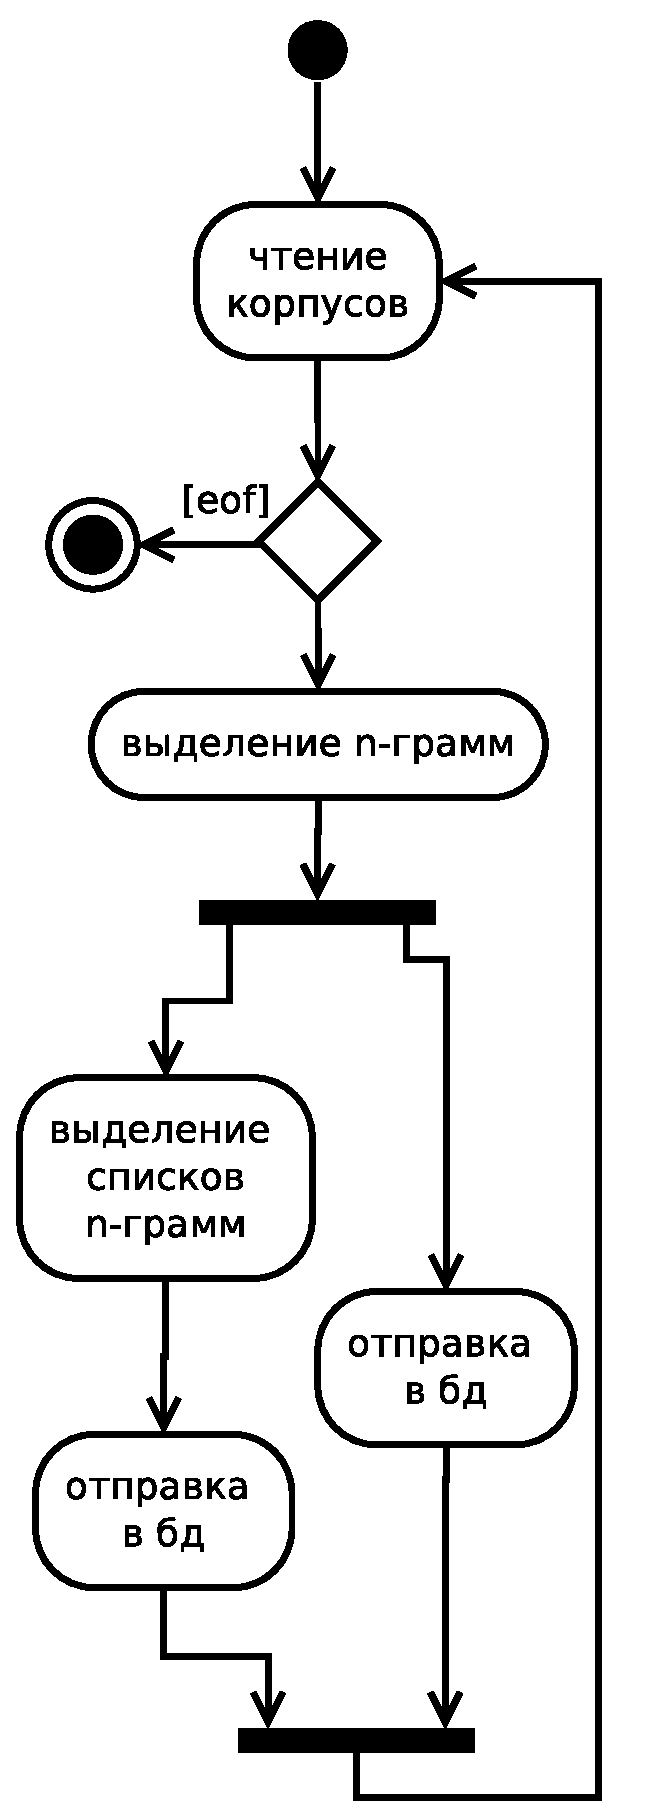
\includegraphics[height=15.0cm]{./vec/arch-reader.eps}
\end{center}
\caption{Диаграмма активности приложения <<читатель>>.}
\end{figure}

Приложение считывает параллельный корпус строка за строкой из двух файлов корпуса одновременно.
После прочтения каждая строка разбивается на слова, по синтаксическим признакам конца слова (пробелы, знаки препинания).
Из списков слов формируются группы $n$-грамм начиная с максимального $n$, 
заканчивая слова.
Одним из принципиальных моментов системы является метод выделения списков $n$-грамм.
Имея список $n$-грамм верхнего уровня, скажем пятого, составить список более низкого уровня 
можно без обращения к~исходной строке. Таким образом, выделения списка занимает время строго 
меньшее чем $O(l^2)$ по длине строки.
Формирование списков  $n$-грамм  и~отправка полученных $n$-грамм в~базу может происходить параллельно.
Сама по~себе отправка представляет собой пару операций: инкремент счетчика заданной $n$-граммы в базе 
и добавление слова множество $n$-грамм.
Обе эти операции также можно проводить параллельно, более того отправку 
в~базу данных может быть осуществлена асинхронно, так как для нас не важен возврат 
результата выполнения команды.
$n$-граммы в списке $n$-граммы отсортированы по убыванию их длин, $n$-граммы одинаковой длинны, 
отсортированы по возрастанию позиции первого слова $n$-граммы в исходном предложении.
Добавление в базу списков $n$-грамм представляет 
собой асинхронную запись каждого списка в базу данных подобно добавлению 
элемента в стек.
Общая схема приложения представлена ниже.
Стрелками показаны потоки данных.
Прерывистыми линиями изображены косвенные связи.

\begin{figured}
		\tikzstyle{dspf} = [rectangle,thick,minimum size=1cm,draw=teal!50!black!50,top color=white,bottom color=teal!50!black!20,font=\itshape]
		\tikzstyle{filef} = [rectangle,rounded corners,thick,minimum size=2.5cm,draw=blue!50!black!50,top color=white,bottom color=blue!50!black!20,font=\itshape]
		\tikzstyle{handlerf} = [rectangle,rounded corners,thick,minimum size=2cm,draw=green!50!black!50,top color=white,bottom color=green!50!black!20,font=\itshape]
		\tikzstyle{dbf} = [rounded rectangle,thick,minimum size=2cm,draw=red!50!black!50,top color=white,bottom color=red!50!black!20,font=\itshape]
		
		\tikzstyle{dbpoolf} = [rounded rectangle,thick,minimum size=1cm,draw=orange!50!black!50,top color=white,bottom color=orange!50!black!20,font=\itshape]
		
		\tikzstyle{dbconf} = [rounded rectangle,thick,minimum size=1cm,draw=orange!50!black!50,top color=white,bottom color=orange!50!black!20,font=\itshape]

		\tikzstyle{corporaf} = [draw=yellow!50!black!70,thick,minimum height=1cm,minimum width=2cm,top color=yellow!20,bottom color=yellow!60!black!20,decorate,decoration={random steps,segment length=3pt,amplitude=1pt}]
	\begin{tikzpicture}[thick, node distance=4cm, text height=1.5ex, text depth=.25ex, auto]
		\node[dspf] 						(dsp)	{Диспетчер};
		\node[filef,	above left of=dsp]	(file)
		{
			\begin{tabular}{c}
				Обработчик 	\\ 
				файлов 	\\ 
				(потоков) 	\\ 
			\end{tabular} 
		};
		\node[corporaf,	left of=file]			(corpora)	{Корпус En, Ru};
		\node[handlerf,	above right of=dsp]	(handler)	
		{
			\begin{tabular}{c}
				Модуль работы	\\ 
				со словами		\\ 
			\end{tabular} 
		};
		\node[dbf,	below right of=dsp]		(db)
		{
			\begin{tabular}{c}
				Модуль \\ 
				работы с БД	\\ 
			\end{tabular} 
		};
		\node[dbpoolf,	below left of=dsp]		(dbpool) {Пул соединений};
		\path[->, yellow!40!black!70] 	(corpora)	edge (file);
		\path[<-, blue] 				(dsp)	edge (file);
		\path[<->, blue] 				(dsp)	edge (handler);
		\path[->, red, dashed] 		(file) 	edge (handler);
		\path[->, blue] 				(dsp)	edge (db);
		\path[->, red, dashed] 		(handler) 	edge (db);
		\path[->, blue] 				(db)	edge (dbpool);
	\end{tikzpicture}
	\fcaption{Схема модулей приложения <<читатель>>. }
\end{figured}

В одной из модификаций этого приложения мы сразу в приложении читателя составляли список сопоставления
$n$-грамм разных языков. Это позволяло несколько разгрузить приложение обработчика кроме того давало
возможность гибко настраивать сопоставление $n$-грамм разного размера.

Полный список сопоставления $n$-грамм представляет собой декартово произведения списков $n$-грамм
на разных языках. Но использование полного списка для $n$-грамм  большого размера является 
не экономичным с точки зрения хранения информации. Тем более, учитывая, стилистические особенности
научного текста, крупные группы слов отражающие сходные понятия в научных текстах находятся
примерно на одинаковом удалении от начала предложения.

Для этого случая нами был разработан следующий подход:
{\renewcommand{\labelenumi}{\alph{enumi})}
	\begin{enumerate}
		\item строить полный список сопоставлений (декартово произведение) для $1$-грамм, то есть слов;
		\item строить $m$-диагональную матрицу для всех остальных $n$-грамм.
	\end{enumerate}
}
$m$ выбирается экспериментально, по умолчанию полагается равным $3$.
Такой подход позволяет снизить количество сопоставляемых $n$-грамм, но повышает вероятность
ошибки обучения системы. 
Как показала практика, не все научные тексты удовлетворяют ограничению представленному выше.
Кроме того, это предположение является ошибочным для текстов иных стилей.
В текущей реализации мы отказались от такого подхода.

\pagebreak

\subsubsection{Обработчик}
Обработчик нужен для обучения модели перевода на основании данных полученных у читателя.

\begin{figure}[H]
	\begin{center}
		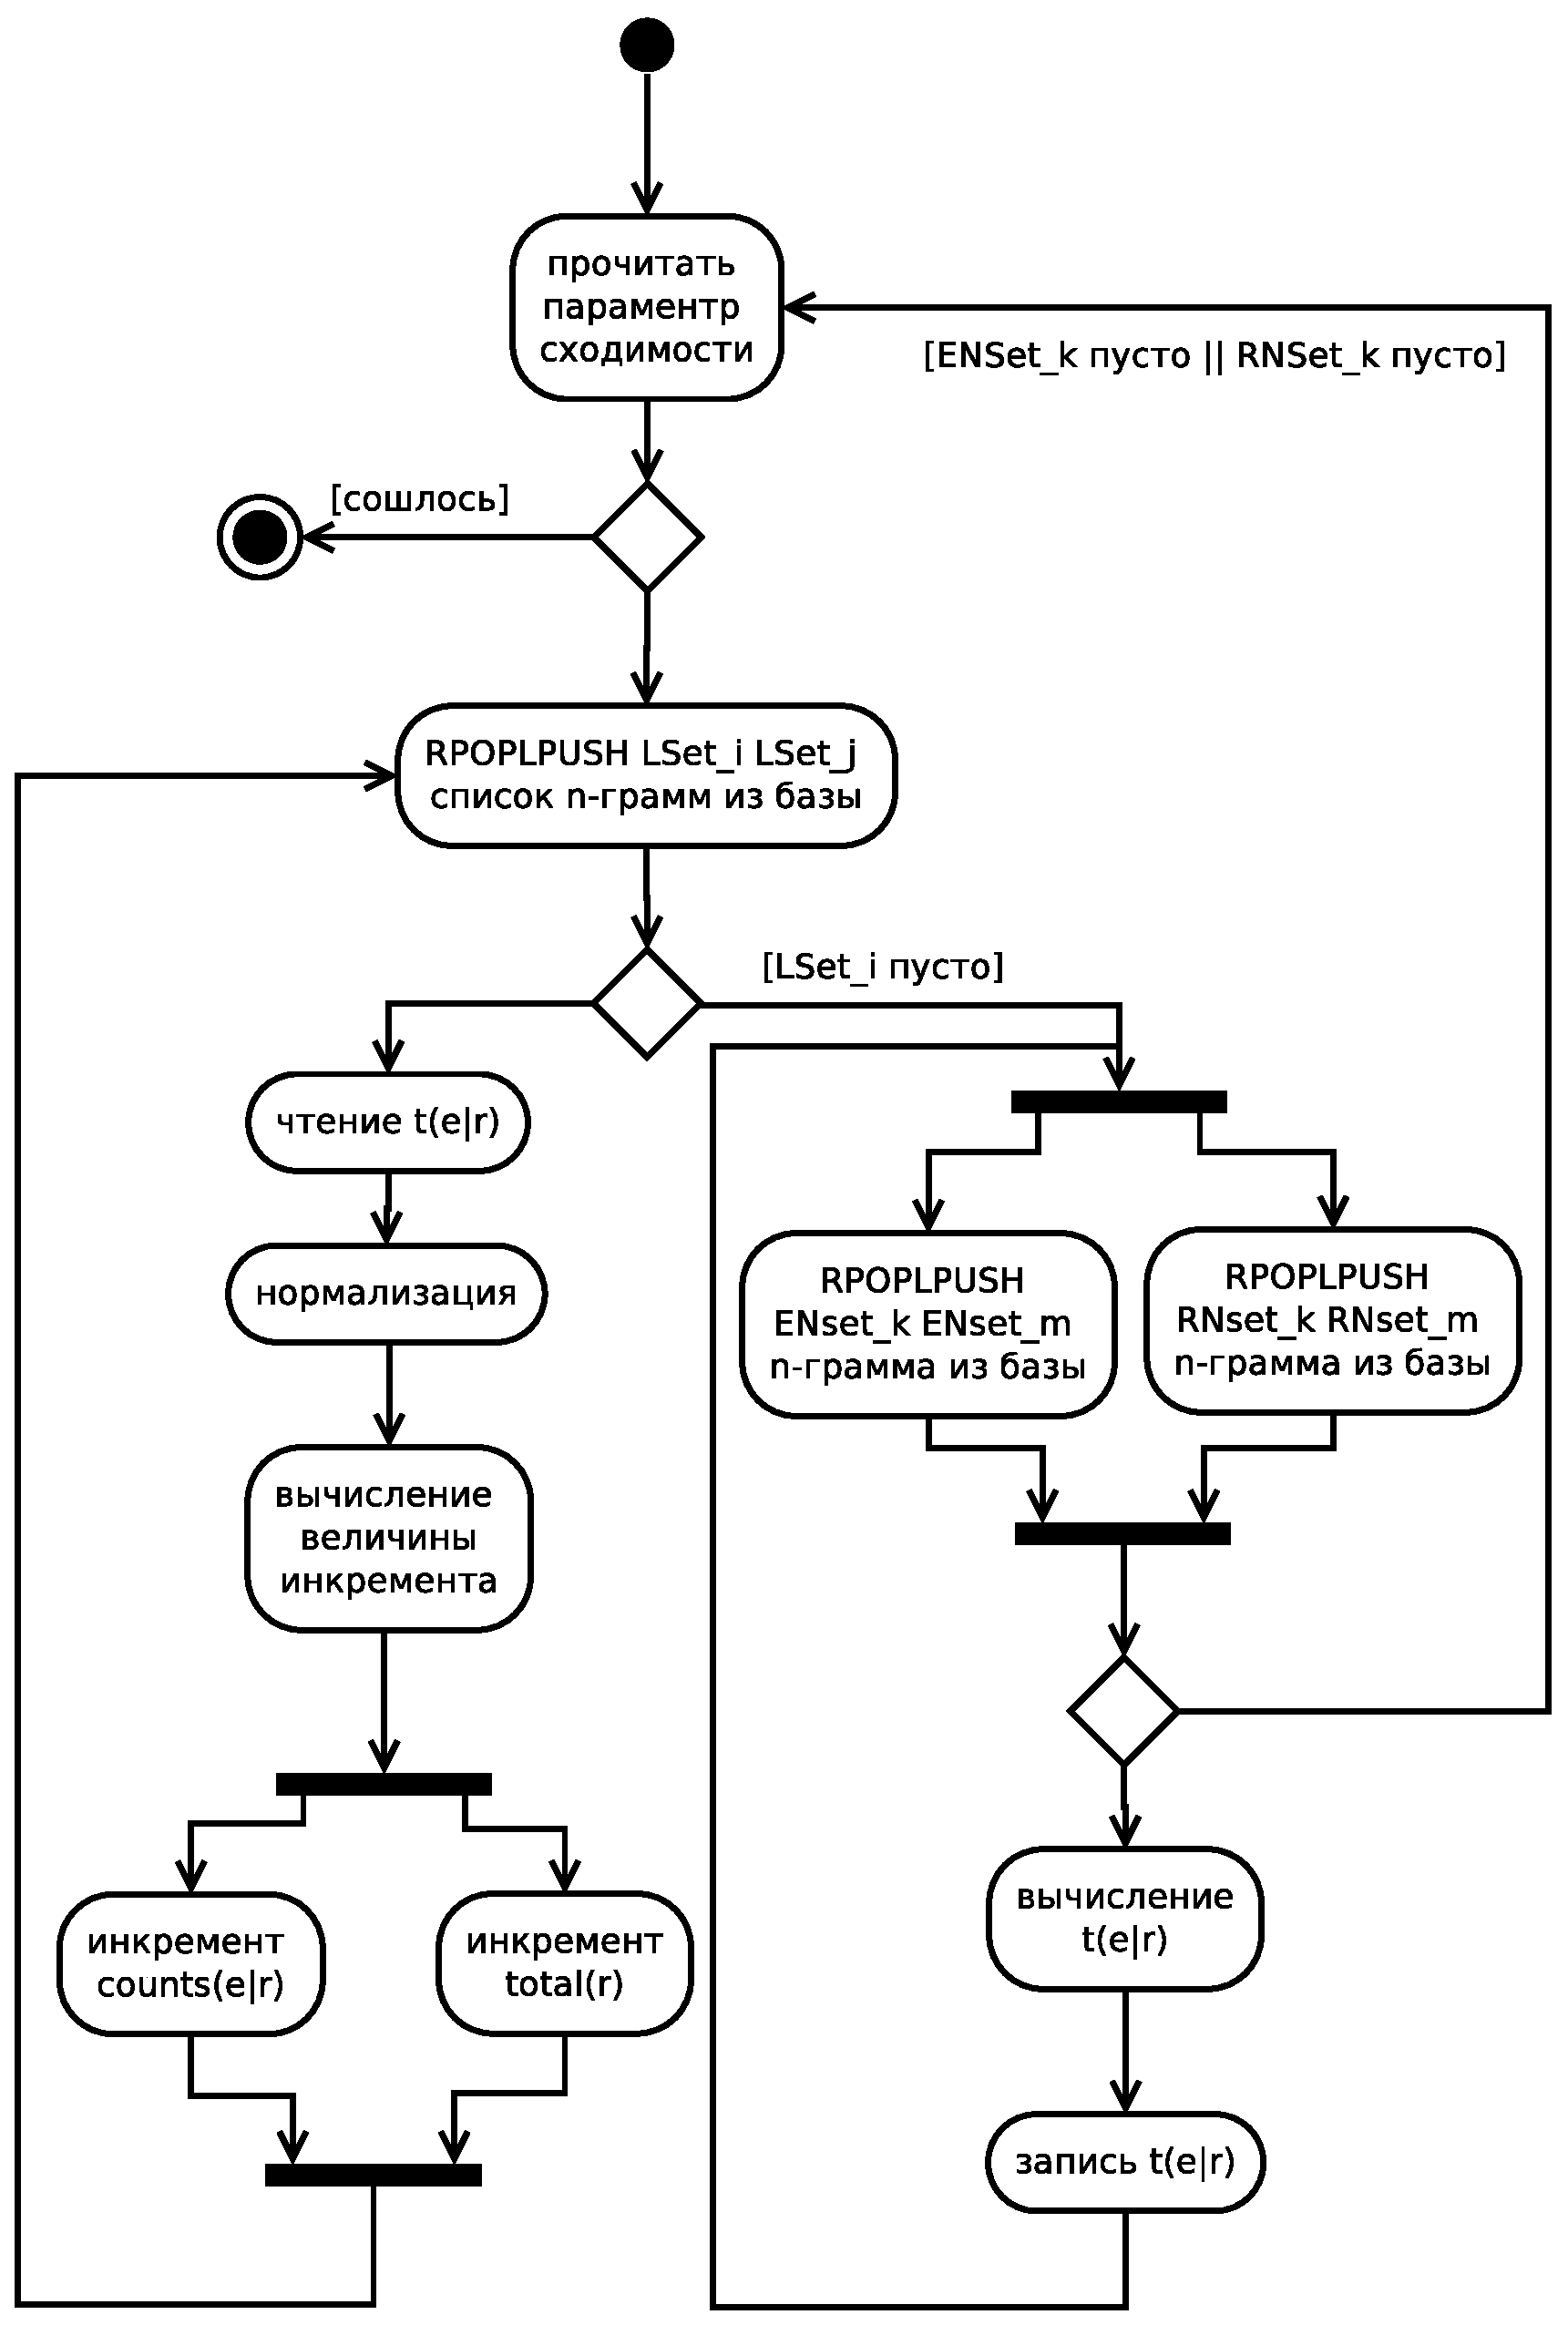
\includegraphics[height=18.0cm]{./vec/arch-handler.eps}
	\end{center}
	\caption{Диаграмма активности приложения <<обработчик>>.}
\end{figure}

\pagebreak

Принцип работы обработчика во многом определяется алгоритмом обучения описанным 
в выше. 
Условие сходимости предлагается не вычислять как математическое неравенство.
Как показала практика на текстах ограниченного объема это условие может никогда не выполниться,
тем более нам не столь важен сам факт сходимости, сколько относительные отношения вероятностей
парных соответствий $n$-грамм. 

Важными архитектурными моментами работы приложения 
являются методы доступа к данным. 
Предполагается что все операции на запись данных буду асинхронными.
Операция инкремента величины подсчетов (см. алгоритмы в приложении),
должны быть атомарными и асинхронными. В противном случае, 
если мы используем распределенные вычисления, то данные рискуют быть 
или неверно прочитаны или перезаписаны в неподходящий момент (оптимистическая блокировка).
Использование пессимистической блокировки может привести 
к значительному замедлению при большой конкуренции запросов.

$\mathrm{Lset}_0$ --- пары списков $n$-грамм перемещенные туда читателем.
На момент начала работы обработчика предполагается что это множество не пусто.
На каждом проходе по множеству элемент этого множества считывается в обработчик
и перемещается в $\mathrm{Lset}_1$ (это выполняется как атомарная операция {\tt rpoplpush}).
При каждой $i$-й итерации алгоритма обработчик считывает 
пару списков $n$-грамм из $\mathrm{Lset}_0$ и кладет их в множество $\mathrm{Lset}_{i+1}$.
Ситуация с вычислением вероятности по всем $n$-граммам корпуса аналогична,
за исключением того, что считывание и перемещение ведется сразу по двум множествам.
Тут так же предполагается, что используемая база данных поддерживает 
атомарные операции такого вида.
В противном случае могут возникнуть конфликты записи данных
и есть возможность, что алгоритм будет многократно отрабатывать 
с ограниченным объемом одних и тех же данных.

Использование множеств в данном контексте может показаться странным.
Более того, оно может показать не самым эффективным решением.
Однако это не так. 
Выбор терминологии и структур хранения данных 
был сделан из практических соображений.
В ходе проектирования и промежуточных реализаций системы 
было опробовано много различных вариантов, которые описаны в ниже.

\pagebreak

\begin{figured}
		\tikzstyle{dspf} = [rectangle,thick,minimum size=1cm,draw=teal!50!black!50,top color=white,bottom color=teal!50!black!20,font=\itshape]
		\tikzstyle{filef} = [rectangle,rounded corners,thick,minimum size=2.5cm,draw=blue!50!black!50,top color=white,bottom color=blue!50!black!20,font=\itshape]
		\tikzstyle{handlerf} = [rectangle,rounded corners,thick,minimum size=2cm,draw=green!50!black!50,top color=white,bottom color=green!50!black!20,font=\itshape]
		\tikzstyle{dbf} = [rounded rectangle,thick,minimum size=2cm,draw=red!50!black!50,top color=white,bottom color=red!50!black!20,font=\itshape]
		\tikzstyle{dbpoolf} = [rounded rectangle,thick,minimum size=1cm,draw=orange!50!black!50,top color=white,bottom color=orange!50!black!20,font=\itshape]
		\tikzstyle{dbconf} = [rounded rectangle,thick,minimum size=1cm,draw=orange!50!black!50,top color=white,bottom color=orange!50!black!20,font=\itshape]
		\tikzstyle{corporaf} = [draw=yellow!50!black!70,thick,minimum height=1cm,minimum width=2cm,top color=yellow!20,bottom color=yellow!60!black!20,decorate,decoration={random steps,segment length=3pt,amplitude=1pt}]
	\begin{tikzpicture}[thick, node distance=4cm, text height=1.5ex, text depth=.25ex, auto]
		\node[dspf] 						(dsp)	{Диспетчер};
		\node[handlerf,	above right of=dsp]	(handler)	
		{
			\begin{tabular}{c}
				Вычислительный 	\\ 
				модуль			\\ 
			\end{tabular} 
		};
			\node[filef,	above left of=handler]	(cnt)
				{
					\begin{tabular}{c}
						Вычисление  \\ 
						подсчетов	\\ 
					\end{tabular} 
				};
			\node[filef,	above right of=handler]	(t)
				{
					\begin{tabular}{c}
						Вычисление	\\ 
						$t(\WE|\WR)$	\\ 
					\end{tabular} 
				};
		\node[dbf,	above left of=dsp]		(db)
		{
			\begin{tabular}{c}
				Модуль \\ 
				работы с БД	\\ 
			\end{tabular} 
		};
		\node[dbpoolf,	below left of=db]		(dbpool) {Пул соединений};
		\path[<->, blue] 				(dsp)	edge (handler);
		\path[<->, blue] 				(dsp)	edge (db);
		\path[<->, red, dashed] 		(handler) 	edge (db);
		\path[<->, blue] 				(db)	edge (dbpool);
		\path[<->, blue] 		(handler) 	edge (cnt);
		\path[<->, blue] 		(handler) 	edge (t);
	\end{tikzpicture}
	\fcaption{Схема модулей приложения <<обработчик>>.}
\end{figured}

Выше представлена схема модулей приложения обработчика.
Стрелками показаны потоки данных.
Прерывистыми линиями изображены косвенные связи.

Для системы крайне критично время доступа к базе данных,
так как для всех численных операций база используется 
как временное хранилище данных между итерациями алгоритма обучения.
Именно поэтому мы на архитектурной схеме изображаем
такую техническую деталь как пул соединений.

\pagebreak

\subsubsection{Декодер}

Согласно описанному ранее алгоритму жадного инкрементного 
поиска декодер имеет два режима работы.

В первом режиме работы на вход принимается исходный текст.
Далее ищется ее наиболее вероятный эквивалент, последовательным разбиением 
фразы на $n$-граммы наибольшего размера (аналогично алгоритму системы перевода основанной на примерах в приложении), 
и параллельным поиском их в базе данных.
После того, как эквивалент всего текста был найден, вычисляется 
величина неопределенности текста:

\begin{Large}
\[
	\text{ВН} = 2^{- \left( \frac{1}{S_{\NE}}\sum\limits_{i = 1}^{S_{\NE}} \log_2 P(\NE_i) 
		+ \frac{1}{S_{\WE}}\sum\limits_{j = 1}^{S_{\WE}} \log_2 P(\WR_j|\WE_j) \right) } 
\]
\end{Large}

\begin{itemize}
	\item $\NE$ --- $n$-граммы высокого порядка найденные в созданном тексте;
	\item $S_{\NE}$ --- количество таких $n$-грамм;
	\item $P(\NE)$ --- вероятность $n$-грамм согласно языковой модели (вычисляется как указано раннее);
	\item $\WE$ --- $n$-граммы (слова) как результат перевода согласно модели перевода;
	\item $S_{\WE}$ --- количество таких $n$-грамм (слов);
	\item $P(\WR_j|\WE_j)$ --- вероятность перевода фразы $\WE_j$ на $\WR_j$.
\end{itemize}

Во втором режиме работы на вход принимается исходный текст (ИТ), переводной текст (ПТ)
c предыдущей итерации и величина неопределенности (ВН).
Применяются операции описанные выше для алгоритма жадного инкрементного поиска,
если полученное новое значение имеет меньшую величину неопределенности чем предыдущее,
то оно подается на выход. В~противном случае итерации продолжаются.

Интерфейсная часть декодера представляет собой 
набор отдельных приложений, которые вызывают функции декодера при поступлении 
запросов на перевод. Общая схема декодера представлена ниже.
Стрелками показаны потоки данных.
Прерывистыми линиями изображены косвенные связи.

\begin{figure}[H]
\begin{center}
		\tikzstyle{dspf} = [rectangle,thick,minimum size=1cm,draw=teal!50!black!50,top color=white,bottom color=teal!50!black!20,font=\itshape]
		\tikzstyle{filef} = [rectangle,rounded corners,thick,minimum size=2.5cm,draw=blue!50!black!50,top color=white,bottom color=blue!50!black!20,font=\itshape]
		\tikzstyle{handlerf} = [rectangle,rounded corners,thick,minimum size=2cm,draw=green!50!black!50,top color=white,bottom color=green!50!black!20,font=\itshape]
		\tikzstyle{dbf} = [rounded rectangle,thick,minimum size=2cm,draw=red!50!black!50,top color=white,bottom color=red!50!black!20,font=\itshape]
		\tikzstyle{dbpoolf} = [rounded rectangle,thick,minimum size=1cm,draw=orange!50!black!50,top color=white,bottom color=orange!50!black!20,font=\itshape]
		\tikzstyle{dbconf} = [rounded rectangle,thick,minimum size=1cm,draw=orange!50!black!50,top color=white,bottom color=orange!50!black!20,font=\itshape]
		\tikzstyle{corporaf} = [draw=yellow!50!black!70,thick,minimum height=1cm,minimum width=2cm,top color=yellow!20,bottom color=yellow!60!black!20,decorate,decoration={random steps,segment length=3pt,amplitude=1pt}]
	\begin{tikzpicture}[thick, node distance=4cm, text height=1.5ex, text depth=.25ex, auto]
		\node[dspf] 						(dsp)	{Диспетчер};
		\begin{scope}[node distance=3.0cm]
		\node[handlerf, above of=dsp]	(iface)	
		{
			\begin{tabular}{c}
				Интерфейсный 	\\ 
				модуль			\\ 
			\end{tabular} 
		};
		\end{scope}			

			\node[handlerf, above left of=iface]	(web)	
			{
				\begin{tabular}{c}
					Веб 				\\ 
					приложение			\\ 
				\end{tabular} 
			};
			
			%	\node[dbpoolf,	above left of=web]		(webctl) {Контроллеры};
			%	\node[dbpoolf,	above right of=web]		(url) {Обработчик URL};
			%	\node[dbpoolf,	left of=web]			(webtpl) {Шаблоны};
			%	\node[dbpoolf,	below left of=web]		(webxsl) {XSLT-преобразователь};
			\node[handlerf, above right of=iface]		(rest)	
			{
				\begin{tabular}{c}
					Rest 	\\ 
					приложение	\\ 
				\end{tabular} 
			};
			%	\node[dbpoolf,	above right of=rest]		(restctl) {Контроллеры};
		\node[handlerf, below right of=dsp]	(handler)	
		{
			\begin{tabular}{c}
				Вычислительный 	\\ 
				модуль			\\ 
			\end{tabular} 
		};
			\node[filef, below left of=handler]	(cnt)
				{
					\begin{tabular}{c}
						Начальный  \\ 
						перевод	\\ 
					\end{tabular} 
				};
			\node[filef, below right of=handler]	(t)
				{
					\begin{tabular}{c}
						Улучшение \\ 
						перевода \\ 
					\end{tabular} 
				};
		\node[dbf, below left of=dsp]		(db)
		{
			\begin{tabular}{c}
				Модуль \\ 
				работы с БД	\\ 
			\end{tabular} 
		};
		\node[dbpoolf,	below left of=db]		(dbpool) {Пул соединений};

		\path[<->, blue] 				(dsp)	edge (handler);
		\path[<->, blue] 				(dsp)	edge (db);
		\path[<->, red, dashed] 		(handler) 	edge (db);
		\path[<->, blue] 				(db)	edge (dbpool);
		\path[<->, blue] 		(handler) 	edge (cnt);
		\path[<->, blue] 		(handler) 	edge (t);
		\path[<->, red, dashed] 		(iface.west) edge (db);
		\path[<->, red, dashed] 		(iface.east) edge (handler);
		\path[<->, blue] 				(iface)	edge (dsp);
		\path[<->, blue] 				(iface)	edge (web);
		\path[<->, blue] 				(iface)	edge (rest);
		% \path[<->, blue] 				(webctl)	edge (web);
		% \path[->, blue] 				(webtpl)	edge (web);
		% \path[<->, blue] 				(webxsl)	edge (web);
		% \path[->, blue] 				(url)	edge (web);
		% \path[->, blue] 				(url)	edge (rest);
		% \path[<->, blue] 				(restctl)	edge (rest);
		% \path[<-, red, dashed] 		(restctl) edge (url);
		% \path[<-, red, dashed] 		(webctl) edge (url);
	\end{tikzpicture}
\end{center}
\caption{Схема модулей приложения <<декодер>>.}
\end{figure}

Rest-приложение представляет из себя HTTP RESTful веб-службу.
К ней по определенному адресу поступает HTTP запрос POST вида.
В теле запроса передается исходный текст для перевода,
который отправляется для декодирования.
После первой итерации декодирования Rest-приложение, 
отвечает запросившему клиенту первым <<наихудшим>> вариантом перевода.
Далее не разрывая соединения генерируются другие варианты перевода
и сразу передаются клиенту. Это продолжается пока клиент 
самостоятельно не разорвет соединение.

Веб-приложение представляет из себя обычный веб-ресурс,
где пользователю предлагается ввести исходный текст для перевода.
После осуществления первой итерации перевода, пользователю
будет предложено улучшить полученный вариант перевода.
Количество итераций по улучшению перевода определяет 
в данном случае сам пользователь.


\begin{figure}[H]
	\begin{center}
		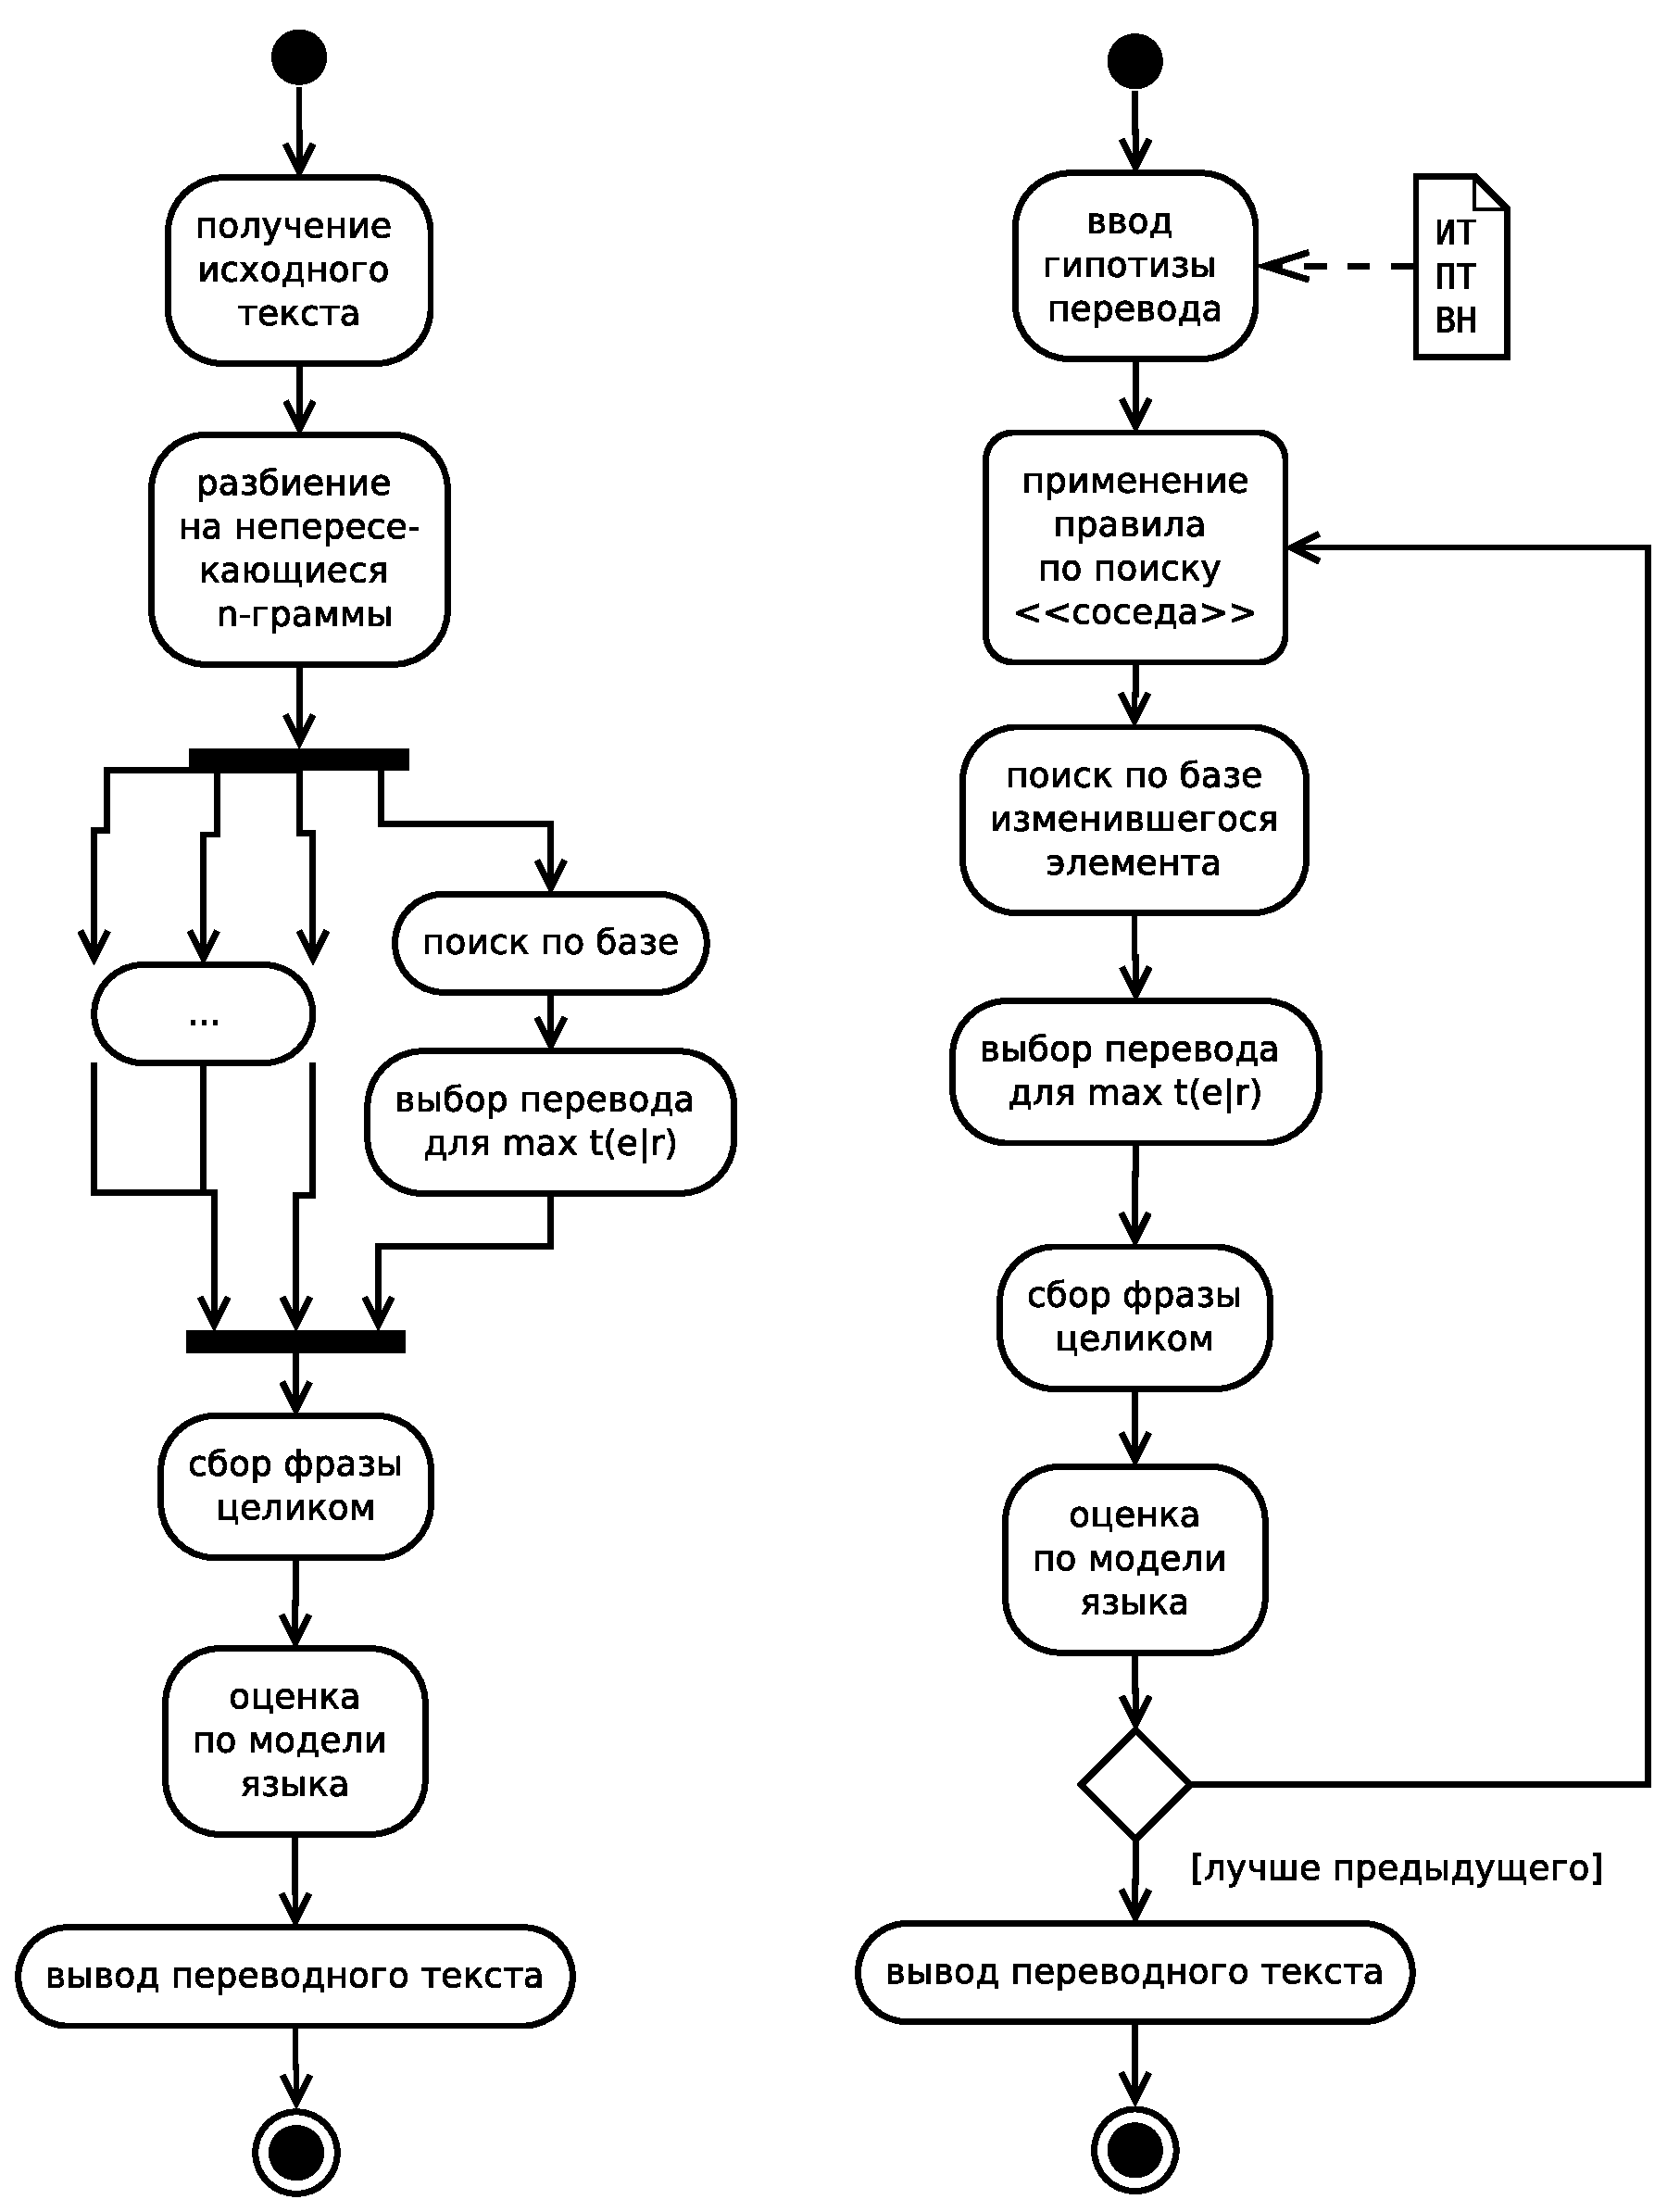
\includegraphics[height=18.0cm]{./vec/arch-decoder.eps}
	\end{center}
	\caption{Диаграммы активности приложения <<декодер>>.}
\end{figure}


\pagebreak

	% Предлагаемый подход
	\subsubsection{Сравнение с решениями других производителей}

На данный момент существует несколько открытых платформ 
для создания систем машинного перевода.
Наиболее крупные из них Moses и Chaski.
Принципы работы этих систем построенных на основе той и другой платформы 
во многом сходны, только с тем отличием, что Chaski позволяет строить распределенные системы. 
Для обучения в обоих случаях используется библиотека GIZA++, однако Chaski включает 
в себя многопроцессорную версию этой библиотеки.

Для тестирования разрабатываемой системы, были созданы еще две ССМП 
на основе Moses и Chaski.
Ниже приведены сравнения этих систем с разработанной.

\begin{dtable}{Сравнение модулей обучения для различных систем.}
	\begin{tabular}{|r|c|c|}
		\hline  \textbf{Система}		& \textbf{Распределенная} 	& \textbf{Отказоуст.} \\  
		\hline  Текущая 				& Да			 			& 	Да \\ 
		\hline  Moses (GIZA++)			& Нет			 			& 	Нет \\ 
		\hline  Chaski (MGIZA++)		& Да			 			& 	Нет \\ 
		\hline 
	\end{tabular} 
\end{dtable}
\begin{dtable}{Сравнение модулей декодирования для различных систем.}
	\begin{tabular}{|r|c|c|c|c|}
		\hline  \textbf{Система}		& \textbf{Распределенная} 	
			& \textbf{Отказоуст.}  & \textbf{Web} & \textbf{Rest}\\  
		\hline  Текущая 				& Да
			& 	{\centering Да  } & Да & Да  \\ 
		\hline  Moses (GIZA++)			& Возможно
			& 	{\centering Нет } & Да & Нет \\ 
		\hline  Chaski (MGIZA++)		& Возможно
			& 	{\centering Нет } & Возможно & Нет \\ 
		\hline 
	\end{tabular} 
\end{dtable}

Самым большим достоинством разработанной системы является то, 
что она ориентирована на перевод текстов исключительно научно-технического характера,
которые имеют явную стилистически подчеркнутую принадлежность к жанру научной прозы.
Такая узкая специализация системы является и основным недостатком.

\pagebreak

			% Сравнение с решениями других производителей

	% Архитектурная часть
	%%%%%%%%%%%%%%%%%%%%%%%%%%%%%%%%%%%%%%%%%%%%%%%%%%%%%%%%%%%%%%%%%%%%%%%%%%%%%%%%
%%%
%%% CODING AND EVAL
%%%

	
\subsection{Реализация ССМП}

\subsubsection{Использование корпуса}

%В ходе работы была попытка протестировать описанные выше подходы на 
%текстах художественной литературы. Для чистоты эксперимента,
%нужно было и обучение системы вести на художественном тексте.

В ходе работы мы попытались построить свой собственный корпус 
для обучения системы на основе <<Лолиты>> Набокова. 
Но проблема заключается в том, что такой корпус крайне сложно выровнять.
Русский и английский варианты местами сильно отличаются.
При попытке разбить на предложения наивным методом (по знакам препинания) 
расхождение возникло на $11$-м предложении.
При попытке разбить на предложения с помощью подробного 
синтаксического анализа, ошибка возникла примерно 
на $200$-м предложении.
Возможно, имеет смысл сначала разбивать текст на абзацы, 
а внутри абзацев разбивать на предложения. 
Ошибка будет иметь меньшее влияние. 
Однако сложно утверждать, 
что такой вариант не обнаружит расхождения в абзацах 
и в любом случае потребуется ручная правка и много времени.
Для маленьких корпусов существуют более сложные методы, 
такие как метод Потемкина-Кедровой \cite{Потемкин:2007}, 
но чаще всего они предполагают наличие заранее подготовленного словаря.

Обычно построение большого корпуса ведется с учетом гипотезы Гайла-Черча, о том, что 
существует прямая зависимость между длинами предложений в исходном тексте и в переводе. 
В рамках данного подхода каждой паре предложений из текстов на разных языках, 
соответствует некоторая характеристика возможности сопоставления. 
Эта характеристика вычисляется на основе разницы длин предложений 
(в символах, включая пробелы) и дисперсии этой разницы. 
Далее, с помощью методов динамического программирования, 
находится такое соответствие предложений, 
при котором характеристики возможности сопоставления максимальны \cite{Липатов:2005}.
Само по себе построение корпуса является самостоятельной задачей корпусной лингвистики.
Потому было принято решение пользоваться уже готовыми корпусами.

\pagebreak

Для  обучения рассматриваемой ССМП использовалась комбинация из нескольких русско-английских корпусов:
{\renewcommand{\labelenumi}{\alph{enumi})}
	\begin{enumerate}
		\item корпус резолюций ООН;
		\item русско-чешско-английский корпус UMC (ÚFAL Multilingual Corpora);
		\item некоторая выборка из Национального корпуса русского языка 
			(была выкачена с веб-сайта корпуса и автоматически сформирована по атрибутам тегов);
		\item некоторая выборка из работы Д. Кнута <<Искусство программирования>> 
			в качестве примера корпуса научных текстов.
	\end{enumerate}
}

Общий объем корпуса составил примерно $180`000$ 
предложений ($5`854`095$ лексических единиц) на каждом из языков.

Важно отметить, что сложно назвать полученную комбинацию корпусом научных текстов,
но за неимением хороших исходных данных пришлось довольствоваться этим.

Большие корпуса научного всего скорее у издательств, и если мы 
захотим развивать систему дальше, 
то можно будет по определенной лицензии эти корпуса приобрести.

Корпуса не обязательно будут выровнены по предложениям, 
но опираясь на свойства научного текста выравнивать 
их самостоятельно достаточно просто. 
Например это можно будет сделать, благодаря наличию формул и 
международных терминов.

\pagebreak
\subsubsection{Средство разработки}

В качестве основного инструментального средства 
используется функциональный язык erlang.

Основные преимущества:
{\renewcommand{\labelenumi}{\alph{enumi})}
	\begin{enumerate}
		\item нет побочных эффектов присущих императивным языкам;
		\item модель легковесных процессов;
		\item удобные средства разработки распределенных приложений;
		\item высокая производительность (меньше чем для~C, но~сопоставима с~C++, 
			при компиляции erlang в машинный код).
	\end{enumerate}
}
	
Очень часто erlang используют для написания высоконагруженных распределенных приложений.
Рассматриваемая система относится именно к таким приложениям.

В ходе выполнения работы как альтернативный вариант рассматривался 
язык программирования python, но после анализ данных производительности 
в рамках данной задачи предпочтение было отдано erlang.

Для увеличения надежности приложений было решено организовать 
взаимодействия процессов c учетом принципов ОТП 
(открытая телекоммуникационная платформа --- OTP, open telecom platform), 
там где это возможно. Диспетчер каждого приложения 
и модуль пула соединения с базой данных имеет 
структуру дерева контроля (<<дерева супервизии>>), как показано ниже на рисунке.
Рабочий процесс может быть обычным вычислительным сервером (в терминах OTP),
или супервизором (более низкого уровня). 
Супервизор в данном случае нужен для контроля за рабочими процессами.
Если у какого либо рабочего процесса произойдет сбой и процесс <<упадет>>, 
то супервизор перезапустит его. 

\begin{figured}
		\tikzstyle{appf} = [rectangle,thick,minimum size=1cm,draw=teal!50!black!50,top color=white,bottom color=teal!50!black!20,font=\itshape]
		\tikzstyle{supf} = [rectangle,rounded corners,thick,minimum size=1cm,draw=blue!50!black!50,top color=white,bottom color=blue!50!black!20,font=\itshape]
		\tikzstyle{wrkf} = [rounded rectangle,thick,minimum size=1cm,draw=red!50!black!50,top color=white,bottom color=red!50!black!20,font=\itshape]
	\begin{tikzpicture}[thick, node distance=4cm, text height=1.5ex, text depth=.25ex, auto]
		\node[appf] 			(app)	{Приложение (в терминах ОТП)};
		\begin{scope}[node distance=2cm]
			\node[supf,below of=app]	(sup)	{Супервизор};
		\end{scope}		
		\begin{scope}[node distance=3.5cm]
			\node[wrkf,below left of=sup]	(wrk1)	{Рабочий процесс $1$};
			\node[wrkf,below right of=sup]	(wrkn)	{Рабочий процесс $n$};
		\end{scope}		
		\node[wrkf,below of=sup]		(wrkd)	{Рабочий процесс $\ldots$};
			
		\path[<->, blue] 				(app)	edge (sup);
		\path[<->, red] 				(sup)	edge (wrk1);
		\path[<->, red] 				(sup)	edge (wrkd);
		\path[<->, red] 				(sup)	edge (wrkn);
	\end{tikzpicture}
	\fcaption{Дерево контроля ОТП.}
\end{figured}

Если сбои будут происходит 
в течение заранее определенного промежутка времени то супервизор 
передаст сигнал о том, что про процесс перестал работать вверх 
по дереву контроля.

Если приложение (в терминах ОТП) контролируется другим супервизором, то процесс повторится снова.
И так пока не дойдет до самого верхнего уровня, что приведет к отказу самого приложения.

\subsubsection{База данных}

В качестве базы данных используется Redis Server.
Ранее были рассмотрены прочие варианты:
\begin{enumerate}
	\item Хранить все словари в памяти, а по окночании скидывать на диск --- очень 
		быстро, но опасно, ибо когда память кончится программа начинает работать не стабильно.
	\item Использовать локальное отображение в файл --- но такой вариант:
	\begin{itemize}
		\item очень медленный;
		\item не масштабируемый.
	\end{itemize}
	\item Попробовали в качестве базы данных использовать Memcache, но оно оказалось 
	медленно, и нет поддержки атомарных операций.
	\item Попробовали в качестве базы данных использовать родные для erlang dts и mnesia, 
		но первая имеет ограничение в размере хранимых данных,
		вторая в количестве хранимых ключей.
\end{enumerate}
В результате долгих поисков и анализа, мы пришли к текущему варианту
Кроме того, Redis версии ниже 2.4 оказался чувствителен к длине ключей и значений. 

Важной особенностью Redis является поддержка атомарных операций обновления,
работа с множествами и списками, работа с хранилищами типа ключ-значение.
Для реализации алгоритмической части были крайне необходимы следующие операции:
\begin{ditemize}
	\item  для работы с $n$-грамами:
	\begin{itemize}
		\item {\tt sadd key value } --- добавить элемент в множество,
		\item {\tt srandmember key  } --- получить случайный элемент множества,
		\item {\tt smove source destination member } --- переместить элемент из одного множества в другое;
	\end{itemize}
	\item для работы со списками $n$-грам:	
	\begin{itemize}
		\item {\tt lpush key value } --- добавление элемента в начало списка,
		\item {\tt rpush key value } --- добавление элемента в конец списка,
		\item {\tt lpop key } --- получение первого элемента списка и его удаление,
		\item {\tt rpop key } --- получение последнего элемента и его удаление,
		\item {\tt rpoplpush srckey dstkey} --- получение и удаление последнего 
			элемента списка {\tt <<srckey>>} с добавлением его в {\tt <<dstkey>>};
	\end{itemize}
	\pagebreak
	\item  для работы с подсчетами и оценкой вероятности:
	\begin{itemize}
		\item {\tt hset key field value } --- установить значение поля,
		\item {\tt hget key field} --- получить значение поля,
		\item {\tt hincrby key field integer} --- увеличить значение поля {\tt <<field>>}
			на~заданную величину {\tt <<integer>>},
		\item {\tt hexists key field } --- проверить существование поля.
	\end{itemize}
\end{ditemize}
Все эти операции имеют константное время доступа.

Учитывая характер системы, достаточно узким ее местом
является скорость доступа к базе данных, особенно, если база является удаленной.
Наличие асинхронных операций записи при вычисления подсчетов в данном 
случае является огромным преимуществом, 
Мы используем параллельный доступ к базе данных. 
Это особенно оказывается критично на синхронных 
операциях чтения.

Для параллельного доступа к базе данных, и исключения блокировок 
мы используем пул соединений с базой данных.
Ниже на рисунке представлено дерево контроля потоков пула соединения. 

\begin{figured}
	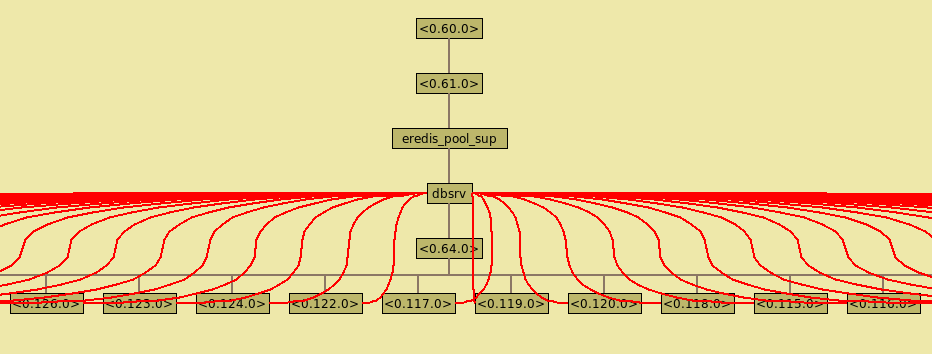
\includegraphics[width=16cm]{./img/practice-dbpool.png}
	\caption{Дерево контроля для пула соединения.}
\end{figured}

\pagebreak

\subsubsection{Арифметика с фиксированной запятой}

В результате деления при осуществлении сбора подсчетов используется вещественное деление.
Для инкремента подсчетов удобно использовать атомарную операцию {\tt hincrby}.
Однако, она работает только с целыми числами. В этом случае мы предлагаем следующий подход.

В качестве вероятности, мы будем использовать числа с фиксированной запятой
по основанию $576460752303423488$ ($2^{59}$). Такое число выбрано не~случайно,
это максимальное положительное число используемое в erlang,
которое может поместиться в машинное слово 64-битной архитектуре.
\[
	Base := 576460752303423488;
\]
%	adiv(X, Y, Base)->   round(Base / Y * X).
\[
	\mathrm{adiv}(X, Y)	\rightarrow \left\lfloor \dfrac{Base}{Y} \cdot X \right\rfloor.
\]
%	amul(X, Y, Base)->   round(X / Base * Y).
\[
	\mathrm{amul}(X, Y)	\rightarrow \left\lfloor \dfrac{X}{Base } \cdot Y \right\rfloor.
\]

При таком подходе возможно появления ошибок гораздо большего порядка, 
чем существующее машинное <<эпсилон>>, но они все равно будут пренебрежимо малы.
Для скорости вычислений и экономии памяти, важно соблюсти
последовательность вычислений.

По проведенном тестам прирост скорости составил примерно 14~раз при~применении 
операции {\tt hincrby} c~числами с~фиксированной запятой, по~сравнению с~последовательными
считывании и~записью в~базу данных.

\subsubsection{Обучение системы}

Основой системы являются базовые алгоритмы моделей IBM 1 и IBM 2 
(можно найти в приложении).
Причем с точки зрения эффективности автор отдает предпочтении IBM 1.
При использовании IBM 2 при падении производительности 
улучшения качества работы системы не замечено было.

В большинстве случаев 
для полной сходимости было достаточно около $10$ итераций. 
Потому в рабочей системе предлагается условие сходимости заменить 
проверкой значения счетчика цикла. 

\paragraph{Инициализация}

В базовом алгоритме указано, что необходимо перед началом его работы 
инициализировать величины $t(\WE|\WR)$ для всех $\WE$ и $\WR$ 
в параллельном корпусе. Логично было бы для этого использовать абсолютную
частоту слова в каждом подкорпусе. Однако, для этого необходимо 
прочитать весь корпус целиком. Если внимательно посмотреть на базовый 
алгоритм, то становится ясно, что от начального значения величин
$t(\WE|\WR)$ ничего не зависит, если они все одинаковы.
В таком случае, можно их инициализировать 
заранее какой-либо константой, например 
в данной работе используется константа равная $0.5$.
 
\paragraph{Возможные ошибки}

Очень важным моментом реализации алгоритма обучения является то,
что оценка вероятности модели и вычисления подсчетов должны происходить
сразу по всему корпусу текстов.

На начальных этапах реализации системы нами была допущено серьезная ошибка.
Приложения читателя, проходила по корпусу и считывало 1000 строк.
После этого эта тысяча строк отправлялась на обработки и по ней строилась модель
перевода. Затем считывалась следующая порция строк.

В результате этих действий подсчеты вычислялись только для локального набора строк,
и затем по ним вычислялась вероятность переводных соответствий и перезаписывала 
вероятность вычисленную ранее.

После окончания работы алгоритма обучения мы получали вероятности 
переводных соответствий обученные только на последней тысяче строк, 
с некоторым влиянием остального корпуса.

Установить ошибку удалось только после запуска алгоритма в предельном случае
на корпусе состоящим из двух строк, при проходе полного алгоритма
обучения на каждой из них.

\pagebreak
\subsubsection{Реализация интерфейсов декодера}

Рассматриваемая система обладает тремя видами интерфейса:
\begin{itemize}
	\item консольные;
	\item простой веб-интерфейс;
	\item rest-интерфейс.
\end{itemize}

Консольное приложение является стандартным отладочным интерфейсом ОТП приложений.
Для перевода достаточно просто  вызывать соответствующую функцию модуля.

Веб-интерфейс декодера выполнен в виде отдельного ОТП приложения и представляет
из себя полноценный веб-ресурс, реализованный с помощью библиотеки mochiweb.

Мы не будем в работе приводить как внешне выглядит клиентская часть Веб-приложения,
которая отображается в браузере, так как она представляет собой всего лишь текстовый элемент ввода,
две кнопки (<<перевести>> и <<улучшить перевод>>), и текстовый элемент вывода.

Важнейшей частью Веб-приложения является XSLT-преобразователь.
В данном случае он был написан на С c использованием libxml2 и libxslt.
Из erlang он вызывается как порт-сервер. На вход подается строка XML 
которая содержит в себе данные (в нашем случае, это перевод исходного текста в случае ответа на запрос)
и шаблон XSL, в котором описано как данные передавать.
Для увеличения быстродействия XSLT преобразователь (на стороне кода на C) 
использует хэш-таблицу, в которой записываются использованные ранее XSL шаблоны. 
Сделано для того, чтобы не загружать при повтором обращении каждый шаблон снова.
В рамках проекта было реализовано две версии преобразователя c запоминанием шаблонов и без него.
Версия без хэш-таблицы работает медленнее, но удобнее при <<горячей замене>> шаблона 
уже на работающем коде.
Кроме того, преобразователь является не блокирующим и при одновременных обращениях
вызывается параллельно. Последнее дает прирост производительности 
при наличие нескольких процессоров или ядер.

Rest-интерфейс декодера также выполнен в виде отдельного ОТП приложения и представляет
из себя полноценный веб-ресурс реализованный с~помощью библиотеки mochiweb.

После поступления POST запроса приложению, оно начинает 
передавать текстовый (Content-Type: text/plain) 
HTTP (chunked) поток с~наиболее вероятными вариантами перевода. 
Этот поток будет передаваться до тех пор, 
пока клиент не закроет соединение, 
или не будут перебраны все варианты улучшения перевода.

Поток представляет из себя набор чанков в рамках спецификации протокола HTTP 1.1.
Каждый чанк содержит количество передаваемых байт и последовательность передаваемых данных.

Каждая строка полного перевода исходного текста передается 
в отдельном чанке и обязательно заканчивается 
символом перевода строки.

В отличие от web-интерфейса в этом случае клиенту не нужно будет самому
запрашивать улучшение перевода. Самый первый <<жадный>> вариант перевода 
передается в первом чанке потока.

\pagebreak

	% Реализация
	%%%%%%%%%%%%%%%%%%%%%%%%%%%%%%%%%%%%%%%%%%%%%%%%%%%%%%%%%%%%%%%%%%%%%%%%%%%%%%%%
%%%
%%% EVAL
%%%

\subsection{Тестирование разработанной ССМП}

\subsubsection{Оценка качества перевода}

Для оценки качества перевода достаточно взглянуть на таблицу ниже.
В ней приведены переводы одного и того же фрагмента для различных 
статистических систем машинного перевода.

\begin{dtable}{Различные переводы исходного текста}
		\begin{tabular}{|r|p{10cm}|}
			\hline  Исходный текст 		& adopted at the 81st plenary meeting \\ 
			\hline  Проф. переводчик 	& принята на 81-м пленарном заседании \\ 
			\hline  Moses 				& приняли на 81 полный встречи \\ 
			\hline  Google-переводчик 	& принятой на 81-е пленарное заседание \\ 
			\hline  Данная система 		& принята без голосования на 81 пленарном заседании в Брюсселе \\ 
			\hline 
	\end{tabular} 
\end{dtable}

Все правильно, заседании было в Брюсселе, но в исходном тексте этого 
не~было. Однако не совсем корректно сравнивать системы, обученные на разных
корпусах текстов. Потому мы будем использовать систему машинного перевода
основанную на пакете Moses (декодировщик Moses и обучающая система GIZA++),
обученную на том же самом входном корпусе, что и наша система.

Для оценки качества перевода существует набор формальных метрик.
\begin{itemize}
	\item BLEU (Bilingual Evaluation Understudy);
	\item METEOR (Metric for Evaluation of Translation with Explicit ORdering);
	\item NIST (названа по имени университета National Institute of Standards and Technology);
	\item WER (Word error rate).
\end{itemize}

Чаще всего системы машинного перевода оценивают по метрике BLEU:
\begin{itemize}
	\item высокая корреляция с оценкой человека;
	\item для оценки требуется готовый перевод тестовых предложений, выполненный профессиональным переводчиком.
\end{itemize}

\[
	\mathrm{BLEU} = Bp \cdot e^{ \left(  \sum\limits_{n=1}^{N} W_n \log(p_n) \right) }
\]\[
	Bp = \left\lbrace 
		\begin{array}{cc}
			1, &  l_c > l_h;\\ 
			e^{\left(1 - \frac{l_h}{l_c}\right)}, &  l_c \le l_h.\\ 
		\end{array} 
	\right.
	\quad \text{ и }\quad
	p_n =
		\dfrac{\sum\limits_{C \in S_c}  \sum\limits_{\eta_c \in C} \text{\it число}_{\text{среза}}(\eta_c) }
			{\sum\limits_{C \in S_c}  \sum\limits_{\eta_c \in C} \text{\it число}(\eta_c) }
\]

\begin{itemize}
	\item $S_c$ --- множество кандидатов на перевод;
	\item $C$ --- кандидат на перевод; 
	\item $\eta_c$ --- $n$-грамма кандидата на перевод;
	\item $l_c$ --- длинна кандидата перевода;
	\item $l_h$ --- длинна экспертного перевода (выполненного человеком);
	\item $W_n = \dfrac{1}{N}$ --- вес, для метрик основанных на BLEU, но не эквивалентных ей, может отличаться для каждого $n$, например NIST назначает больший вес более редким $n$-граммам;
	\item $N = 4$, $n$-грамность оценки.
\end{itemize}

Таким образом, BLEU есть взвешенное среднее числа совпадений
$n$-грамм (слов) кандидата и $n$-грамм в переводе эксперта. 
Метрика является инвариантом порядка $n$-грамм, важно наличие совпадений \cite{Кан:2011}. 
Чем выше значение метрики BLEU, тем перевод хуже.

Метрики NIST и METEOR основаны на BLEU, WER --- на вычислении расстояния Левенштейна.

Для оценки перевода системы мы использовали метрику BLEU.
Для подсчета метрики было выделено 1024 предложений в качестве примеров экспертного перевода, 
и 1024 предложений было переведено рассматриваемой системой МП. 
Для этого набора предложений метрика BLEU = 0.243 для единственной итерации работы декодера,
и 0.209 для лучшего варианта из 100  полученного в результате нескольких итераций.
Система МП, построенная на основе пакета Moses,
 дает метрику BLEU = 0.209 для модели IBM 3 и BLEU = 0.173 для модели IBM 5.

\begin{dtable}{Оценки перевода текста}
	\begin{tabular}{|r|r|}
		\hline  \textbf{Система}	&	\textbf{BLEU}  \\ 
		\hline  Текущая (1)			&	0.243 \\ 
		\hline  Текущая (100)		&	0.209 \\ 
		\hline  Moses (IBM 3)		&	0.201 \\ 
		\hline  Moses (IBM 5) 		& 	0.173 \\ 
		\hline 
	\end{tabular} 
\end{dtable}

Высокие значения метрики BLEU показывают, что система проявляет 
себя не в лучшем свете на тестовом корпусе, однако сам корпус
весьма отличается отличается от тех для которых создана данная система.

Существует целый ряд неформальных способов оценки систем машинного перевода.
Чаще всего используют технику <<обратного перевода>>. 
\begin{itemize}
	\item исходный отрывок переводят системой c языка $L_1$ на язык $L_2$;
	\item полученный отрывок переводят в обраПритную сторону c языка $L_2$ на язык $L_1$.
	\item сравнивают два варианта отрывка на языке 	$L_1$ и по их близости судят о качестве перевода.
\end{itemize}
На наш взгляд такой метод оценки не является вполне корректным в случае статистических систем.
Так как согласно уравнению Байеса, в итоге мы оцениваем только модель языка используемой системы.
Более того при многократном применении <<обратного перевода>> к одному и тому же отрывку,
с некоторой итерации перевод на $L_1$ и на $L_2$ перестанут меняться.

\pagebreak

\subsubsection{Оценка скорости}

\paragraph{Оценка скорости обучения}

Ниже мы сравним скорости обучения и работы трех систем машинного перевода.
Для того чтобы показать разницу распределенных (многопоточных) и не распределенных систем
эксперименты проводились на разных машинах.
Для тестирования рассматриваемой системы было на каждой машине запускались 
соответствующие приложения (читатель и обработчик), пропорционально числу ядер процессоров.
Тестирование как и ранее проводилось на смешанном корпусе описанном выше.

Высокая скорость текущей (представленной в работе) системы 
во многом объясняется ее простотой. 
Однако, для более крупных корпусов текста, скорость обучения может оказаться критичной.

\textbf{Оценка скорости обучения на одном и том же корпусе.} \\

\begin{dtable}{Оценка скорости обучения, процессор: Intel Core2 Duo, 1 ядро 64 бит, ОП 4Гб, ФС:~ext4}
	\begin{tabular}{|r|r|}
		\hline  \textbf{Система}		& \textbf{Время, ч} \\  
		\hline  Текущая (1)				&	$ \approx $ 5   \\ 
		\hline  Moses (GIZA++)			&	$ \approx $ 25  \\ 
		\hline  Chaski (MGIZA++)		&	$ \approx $ 26  \\ 
		\hline 
	\end{tabular} 
\end{dtable}

\begin{dtable}{Оценка скорости обучения, процессор: Intel Xeon E5506, 8 ядер 64 бит, ОП 10Гб, ФС:xfs}
	\begin{tabular}{|r|r|}
		\hline  \textbf{Система}	& \textbf{Время, ч} \\ 
		\hline  Текущая (1)			&	$ \approx $ 1 	\\
		\hline  Moses (GIZA++)		&	$ \approx $ 22 	\\
		\hline  Chaski (MGIZA++)	&	$ \approx $ 3 	\\ 
		\hline 
	\end{tabular} 
\end{dtable}

\paragraph{Оценка скорости перевода}

Скорость перевода будем оценивать в микросекундах. 
Причем, скорость запуска декодера (Moses стартует в течение минуты на Intel Core2 Duo) 
и время на прочие накладные вычисления учитывать не будем. \\

\begin{dtable}{Оценка скорости перевода, процессор: Intel Core2 Duo, 1 ядро 64 бит, ОП 4Гб, ФС: ext4}
	\begin{tabular}{|r|r|}
		\hline  \textbf{Система}	&	Время, $\mu$с \\ 
		\hline  Текущая (1)			&	1132 \\ 
		\hline  Текущая (100)		&	7108124  \\ 
		\hline  Moses (IBM 3)		&	$\approx$ 10000000\\ 
		\hline  Moses (IBM 5) 		& 	$\approx$ 30000000 \\ 
		\hline 
	\end{tabular} 
\end{dtable}

\begin{dtable}{Оценка скорости перевода, процессор: Intel Xeon E5506, 8 ядер 64 бит, ОП 10Гб, ФС: xfs}
	\begin{tabular}{|r|r|}
		\hline  \textbf{Система}	&	Время, $\mu$с \\ 
		\hline  Текущая (1)			&	1012 \\ 
		\hline  Текущая (100)		&	1119024  \\ 
		\hline  Moses (IBM 3)		&	$\approx$ 5000000\\ 
		\hline  Moses (IBM 5) 		& 	$\approx$ 6000000 \\ 
		\hline 
	\end{tabular} 
\end{dtable}

Как можно заключить из приведенных тестов использование параллельных вычислений позволяет 
достичь значительного прироста производительности на этапе обучения системы машинного перевода.

На этапе декодирования особенный рост наблюдать трудно. 
Это будет весьма заметно на большом количестве одновременных запросов.
 
\pagebreak

		% Тестирование


		% Практическая часть
		
\pagebreak

            % основная часть
        %%%%%%%%%%%%%%%%%%%%%%%%%%%%%%%%%%%%%%%%%%%%%%%%%%%%%%%%%%%%%%%%%%%%%%%%%%%%%%%%
%%%
%%% Расчет затрат на разработку
%%%

%%%%%%%%%%%%%%%%%%%%%%%%%%%%%%%%%%%%%%%%%%%%%%%%%%%%%%%%%%%%%%%%%%%%%%%%%%%%%%%%
%%%
%%% Общие положения
%%%

\pagesection{Экономическая часть}

	%%%%%%%%%%%%%%%%%%%%%%%%%%%%%%%%%%%%%%%%%%%%%%%%%%%%%%%%%%%%%%%%%%%%%%%%%%%%%%%%
%%%
%%% Общие положения
%%%

\subsection{Введение}

По мере того как расширяется информатизация современного общества, 
возрастает значение прикладной (вычислительной, компьютерной, инженерной) 
лингвистики, науки, находящейся на стыке глубоко человечной, гуманитарной 
науки лингвистики (языкознания), изучающей законы развития 
и пользования могучим средством мышления и коммуникации --- языком, --- 
и компьютерного знания, с помощью которого машине передастся 
все большая часть интеллектуального труда человека \cite{Марчук:2000}.

В данной главе будет рассмотрена экономическая сторона вопроса. 
Вначале будет построена сетевая модель работ над проектом и её графическое представление. 
Будут рассчитаны ранние и поздние сроки начала и завершения работ над проектом, 
найден критический путь и его продолжительность, вероятность завершения 
комплекса работ по проекту в срок. После этого будет рассчитана сумма 
расходов на разработку проекта. Будет подсчитана цена разработанной системы, 
капитальные вложения, связанные с её внедрением, а также расходы, 
связанные с её эксплуатацией.


	%%%%%%%%%%%%%%%%%%%%%%%%%%%%%%%%%%%%%%%%%%%%%%%%%%%%%%%%%%%%%%%%%%%%%%%%%%%%%%%%
%%%
%%% Введение
%%%

\subsection{Построение сетевой модели}

Сложность и~комплексность разработки и~реализации описанного проекта, 
необходимость параллельного выполнения работ, 
зависимость начала многих работ от результатов других, 
значительно осложняют планирование разработки.

При наличии множества взаимосвязанных работ,
наиболее удобными являются системы сетевого планирования и~управления (СПУ).
Они основаны на~применении сетевых моделей планируемых процессов, 
которые допускают использование современной вычислительной техники. 

Сетевые модели планируемых процессов позволяют быстро определить 
последствия различных вариантов управляющих 
воздействий и~находить наилучшие из них. 

СПУ дают возможность своевременно получать достоверную информацию о~состоянии дел, 
о возникших задержках и~возможностях ускорения хода работ, 
концентрируют внимание на~<<критических>> работах, 
определяющих продолжительность проведения разработки в целом, 
заставляют совершенствовать технологию и~организацию работ, 
непосредственно влияющих на~сроки проведения разработки, 
помогают составлять рациональные планы работ.

\subsubsection{Перечень работ и~событий}

Составим полный перечень событий и~работ сетевой модели. 
Каждая работа имеет определенную продолжительность. 
Однако не всегда заранее известно точное время выполнения работ, 
поэтому дадим продолжительности каждой работы две вероятностные оценки:   

\begin{itemize}
	\item минимальную (оптимистическую) --- $t_{min}$;
	\item максимальную (пессимистическую) --- $t_{max}$.
\end{itemize}

Эти величины являются исходными для расчета ожидаемого времени выполнения работ:  .
\[
	t_{\text{ожидаемое}} = \dfrac{3 \cdot t_{min} + 2 \cdot t_{max} }{5}
\]

Рассчитаем дисперсии работ по формуле:   
\[
	\delta^2 = \left(  \dfrac{ t_{max} - t_{min} }{5} \right)^2
\]




\pagebreak


{ \footnotesize \sffamily 
\begin{spacing}{1.2}
\begin{center}
	\captionsetup{font=rm,justification=raggedleft, singlelinecheck=false,font=small}
	\newcommand{\headlinetext}{
		\textbf{№} &	\textbf{Наименование события}  &	\textbf{Код работы}  &	\textbf{Наименование  работы} 
		& $\mathbf{t_{min}}$ &	$\mathbf{t_{max}}$ & $\mathbf{t_{\text{\textbf{ож}}}}$ & $\mathbf{\delta^2}$
	}
	\newcommand{\captiontext}{
		Перечень работ и~событий, 
			$t_{min}$, $t_{max}$,
				$t_{\text{ож}}$ измеряются в днях.
	}
	\begin{longtable}{|r|m{3.8cm}|c|m{4cm}|r|r|r|r|}
		\caption{\captiontext}\\
		\hline
			\headlinetext
		\endfirsthead
			\captionsetup{labelformat=continued}
			\caption{\captiontext}\\
		\hline
			\headlinetext
		\endhead
		\hline
		\hline
				0 &
				Начало работ &
				0 --- 1  &
				Анализ проблемы и~составление плана-графика &
				2 & 5 & 3.8 & 0.16 \\
		\hline
			\multirow{3}{*}{1} &
			\multirow{3}{4cm}{Завершение анализа и~составления плана} &
			1 --- 2  &
			Исследование существующих статистических систем машинного перевода &
			4 & 10 & 6.4 & 1.44 \\
		\cline{3-8} & &
			1 --- 3  &
			Изучение математических основ построения статистических систем машинного перевода &
			10 & 20 & 14.0 & 4.0 \\
		\cline{3-8} & &
			1 --- 4  &
			Изучение лингвистических основ машинного перевода &
			7 & 10 &  8.2 & 0.36 \\
		\cline{3-8}	& &
			1 --- 5  &
			Изучение возможных вариантов хранения данных в рамках задачи машинного перевода &
			3 & 4 & 3.4 & 0.04 \\
		\hline
			2 &
			Завершение исследования существующих систем &
			2 --- 6  &
			Составление требований и~ограничений системы &
			1 & 2 & 1.6	 &  0.04 \\
		\hline
			\multirow{2}{*}{3}  &
			\multirow{2}{4cm}{Завершение изучения математических основ  построения статистических систем машинного перевода } &
			3 --- 7  &
			Разработка численного алгоритма обучения системы &
			5 & 7 & 5.8 & 0.16 \\
		\cline{3-8}	& &
			3 --- 8  &
			Разработка алгоритма поиска верного варианта перевода на~основе обученной модели &
			6 & 8 & 6.8 & 0.16 \\
		\hline
			\multirow{2}{*}{4}  &
			\multirow{2}{4cm}{Завершение изучения лингвистических основ машинного перевода} &
			4 --- 9  &
			Составление требований к~входным данным численного алгоритма &
			1 & 2 & 1.6	 &  0.04 \\
		\cline{3-8}	& &
			4 --- 8  &
			Составление требований к~выходным данным алгоритма поиска  &
			1 & 2 & 1.6	 &  0.04 \\
		\hline
			5 &
			Завершение изучения возможных вариaнтов хранения данных  &
			5 --- 7 &
			Разработка структуры хранения данных &
			2 & 3 & 2.4 & 0.04 \\
		\hline
			6 &
			Завершение составления требований к~системе на~основе аналогов  &
			6 --- 10  &
			Разработка распределенной архитектуры &
			3 & 4 & 3.4 & 0.04 \\
		\hline
			7 &
			Завершение разработки численного алгоритма и~структру хранения данных &
			7 --- 10  &
			Разработка работающей обучающейся модели на~тестовых входных данных &
			5 & 7 & 5.8 & 0.16 \\
		\hline
			8 &
			Завершение  разработки алгоритма поиска и~выработки требований к~выходным данным &
			8 --- 13 &
			Разработка работающего  поискового модуля на~тестовых входных данных &
			6 & 9 & 7.2 & 0.36 \\
		\hline
			9 &
			Завершение составления требований к~входным данным численного алгоритма &
			9 --- 11  &
			Подбор нужных корпусов текстов (корпуса текста все еще остаются тестовыми, 
			но составляются на~основе реальных данных) &
			5 & 7 & 5.8 & 0.16 \\
		\hline
			10 &
			Окончание разработки распределенной архитектуры и~ и~модели обучающейся на~тестовых входных данных&
			10 --- 12  &
			Разработка распеределенной обучающейся системы &
			2 & 4 & 2.8 & 0.16 \\
		\hline
			11 &
			Окончание подбора нужных корпусов текстов &
			11 --- 12  &
			Разработка алгоритмов предварительной обработки входных корпусов текста &
			1 & 2 & 1.4 & 0.06 \\
		\hline
			12 &
			Окончание разработки распеределенной обучающейся системы 
				и алгоритмов предварительной обработки входных данных&
			12 --- 13  &
			Корректировка  системы с~учетом входных данных &
			1 & 2 & 1.4 & 0.06 \\
		\hline
			13 &
			Окончание корректировки обучающейся системы  и~разработки работающего  поискового модуля &
			13 --- 14  &
			Тестирование приложения в совокупности отладка всей системы &
			10 & 15 & 12.0 & 1.0 \\	
		\hline
			14 &
			Завершение отладки &
			14 --- 15  &
			Прогон системы на~реальных корпусах текста &
			1 & 2 & 1.5 & 0.06 \\	
		\hline
			15 &
			\multicolumn{7}{l|}{			Завершение работ} \\	
		\hline
	\end{longtable} 
	\vspace{1cm}
\end{center}
\end{spacing}
}

\subsubsection{Графическое представление сетевой модели}

\begin{dfigure}{Сетевой граф работ и~критический путь.}
	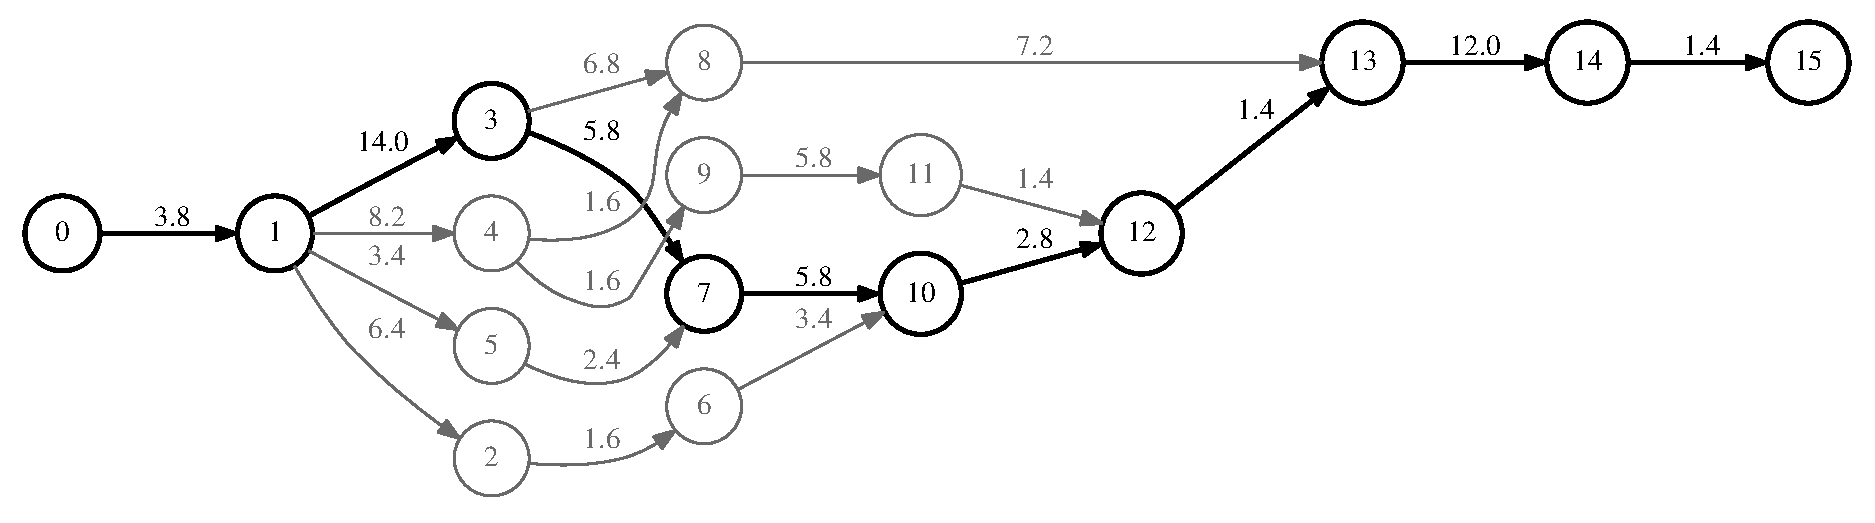
\includegraphics[width=15cm]{./vec/net-model.eps}
\end{dfigure}

Построенный граф состоит из $15$ событий (вершины графа).
Дуги графа --- работы. Каждая дуга графа подписана~сверху соответствующей~ей
продолжительностью работ.

Построенный граф удовлетворяет условию независимости событий $i$ от
события $j$ для все $i > j$. Выполнение этого условия очевидно, так~как~ни одна
дуга не заканчивается в вершине с~номером, меньшим, чем номер вершины
из которой это дуга начиналась. Это позволяет корректно выполнять
дальнейшие расчеты.

\subsubsection{Расчет параметров сетевой модели}

Рассчитаем некоторые характеристики сетевой модели. Характеристики
сетевой модели позволяют определить степень напряженности всего
комплекса работ в целом и~каждой работы в отдельности, а также принять
решение о~перераспределении ресурсов.

Для всех работ рассчитаем следующие показатели:

\begin{itemize}
	\item  ранний срок~начала работы:
		$
			t_{\text{рн}, i - j}  = \max\limits_ {k< i} \left(  t_{\text{ожидаемое}, k - i}  + t_{\text{рн}, k - i} \right)
		$;
	\item ранний срок~окончания работы:
		$
			t_{\text{рo}, i - j}	 = t_{\text{рн}, i - j} + t_{\text{ожидаемое}, i - j} 
		$;
	\item  поздний срок~начала работы: 
		$
			t_{\text{пн}, i - j}	 = t_{\text{по}, i - j} - t_{\text{ожидаемое}, i - j} 
		$;
	\item  поздний срок~окончания работы:
		$
			t_{\text{по}, i - j}  = \min\limits_ {k> j}  \left( t_{\text{по}, j - k} - t_{\text{ожидаемое}, j - k}  \right)
		$;
	\item  полный резерв времени:
		$
			r_{\text{п}, i - j} =t_{\text{пн}, i - j}	 - t_{\text{рн}, i - j}
		$;
	\item  свободный резерв времени: 
		$
			r_{\text{с}, i - j} = t_{\text{рн}, j} - t_{\text{рн}, i} - t_{\text{ожидаемое}, i - j} 
		$.
\end{itemize}

\begin{dsmalltable}{Характеристики сетевой модели, $t$ и~$r$ измеряются в днях.}
	\begin{tabular}{|r|r||r|r||r|r||r|r||r|r|}
		\hline
			Код работы &  $ t_{\text{ож}} $  &
				 $ t_{\text{рн}} $  & $ t_{\text{рo}} $  &
					 $ t_{\text{пн}} $  & $ t_{\text{пo}} $  &
						$ r_{\text{п}} $ & $ r_{\text{с}} $ & 
							$ t_{\text{ож. кр. пути}} $ & $ \delta^2_{\text{кр. пути}}$ \\ 
		\hline
			\textbf{1} &   \textbf{2} & 
				\textbf{3} & \textbf{4} $= 2 + 3$ & 
					\textbf{5} $= 6 - 2$ & \textbf{6} & 
						\textbf{7} $= 5 - 3$ & \textbf{8} & 
							\textbf{9} &  \textbf{10} \\
		\hline 
			\hline  0 --- 1 &$ 3.8$&$ 0.0$&$ 3.8$&$ 0.0$&$ 3.8$&$ 0.0$&$ 0.0 $&$ 3.8$&$0.16$\\
			\hline  1 --- 2 &$ 6.4$&$ 3.8$&$10.2$&$18.0$&$24.4$&$14.2$&$ 0.0 $&$ 0.0$&$0.0 $\\
			\hline  1 --- 3 &$14.0$&$ 3.8$&$17.8$&$ 3.8$&$17.8$&$ 0.0$&$ 0.0 $&$14.0$&$4.0 $\\
			\hline  1 --- 4 &$ 8.2$&$ 3.8$&$12.0$&$15.2$&$23.4$&$11.4$&$ 0.0 $&$ 0.0$&$0.0 $\\
			\hline  1 --- 5 &$ 3.4$&$ 3.8$&$ 7.2$&$17.8$&$21.2$&$14.0$&$ 0.0 $&$ 0.0$&$0.0 $\\
			\hline  2 --- 6 &$ 1.6$&$10.2$&$19.4$&$24.4$&$26.0$&$14.2$&$ 7.6 $&$ 0.0$&$0.0 $\\
			\hline  3 --- 7 &$ 5.8$&$17.8$&$23.6$&$17.8$&$23.6$&$ 0.0$&$ 0.0 $&$ 5.8$&$0.16$\\
			\hline  3 --- 8 &$ 6.8$&$17.8$&$24.6$&$19.6$&$26.4$&$ 1.8$&$ 0.0 $&$ 0.0$&$0.0 $\\
			\hline  4 --- 8 &$ 1.6$&$12.0$&$13.6$&$24.8$&$26.4$&$12.8$&$11.0 $&$ 0.0$&$0.0 $\\
			\hline  4 --- 9 &$ 1.6$&$12.0$&$13.6$&$23.4$&$25.0$&$11.4$&$ 0.0 $&$ 0.0$&$0.0 $\\
			\hline  5 --- 7 &$ 2.4$&$ 7.2$&$ 9.6$&$21.2$&$23.6$&$14.0$&$14.0 $&$ 0.0$&$0.0 $\\
			\hline  6 --- 10&$ 3.4$&$19.4$&$22.8$&$26.0$&$29.4$&$ 6.6$&$ 6.6 $&$ 0.0$&$0.0 $\\
			\hline  7 --- 10&$ 5.8$&$23.6$&$29.4$&$23.6$&$29.4$&$ 0.0$&$ 0.0 $&$ 5.8$&$0.16$\\
			\hline  8 --- 13&$ 7.2$&$24.6$&$31.8$&$26.4$&$33.6$&$ 1.8$&$ 0.4 $&$ 0.0$&$0.0 $\\
			\hline  9 --- 11&$ 5.8$&$13.6$&$19.4$&$25.0$&$30.8$&$11.4$&$ 0.0 $&$ 0.0$&$0.0 $\\
			\hline 10 --- 12&$ 2.8$&$29.4$&$32.2$&$29.4$&$32.2$&$ 0.0$&$ 0.0 $&$ 2.8$&$0.16$\\
			\hline 11 --- 12&$ 1.4$&$19.4$&$20.8$&$30.8$&$32.2$&$11.4$&$11.4 $&$ 0.0$&$0.0 $\\
			\hline 12 --- 13&$ 1.4$&$32.2$&$33.6$&$32.2$&$33.6$&$ 0.0$&$ 0.0 $&$ 1.4$&$0.06$\\
			\hline 13 --- 14&$12.0$&$33.6$&$45.6$&$33.6$&$45.6$&$ 0.0$&$ 0.0 $&$12.0$&$1.0 $\\
			\hline 14 --- 15&$ 1.4$&$45.6$&$47.0$&$45.6$&$47.0$&$ 0.0$&$ 0.0 $&$ 1.4$&$0.06$\\
		\hline	\multicolumn{8}{|r||}{Суммарные время и~дисперсия критического пути:}   &   47.0 &  4.76 \\
		\hline
	\end{tabular} 
\end{dsmalltable}

	
\subsubsection{Анализ сетевой модели}

на~основе посчитанных выше параметров, проведем анализ сетевого
графика. Критически путь включает в себя лишь события с~нулевым запасом времени.
Таким путём является путь из вершин: 
\[
	L_\text{кр} = 0 \rightarrow 1 \rightarrow 3  \rightarrow 7 \rightarrow 10 \rightarrow 12 \rightarrow 13  \rightarrow 14 \rightarrow 15
\]
Суммарное время критического пути составляет $T_\text{кр} = 47$  дней, а его
суммарная дисперсия — $4.76$ дня. 
на~графе критический путь выделен жирными стрелками.

Необходимо, чтобы продолжительность критического пути $T_\text{кр}$
не превышала продолжительности заданного директивного срока $ T_\text{дир}$. 
Если $T_\text{кр} > T_\text{дир}$, то необходимо принять меры по уплотнению графика работ.
В нашем случае директивный срок~создания программного комплекса $T_\text{дир} =63$ дня,\\ 
а продолжительность критического пути $T_\text{кр} = 47$  дней, т.е. $T_\text{кр} < T_\text{дир}$.

Рассчитаем среднеквадратичное отклонение для продолжительности \\
критического пути. 
\[
	\sum\limits_{i-j} \delta^2_{\text{кр. пути}} = 4.76 \Rightarrow  
\]\[
	\Rightarrow  \delta_{\text{кр. пути}} = \sqrt{\sum\limits_{i-j} \delta^2_{\text{кр. пути}}} = \sqrt{4.76} \approx 2.181742422927143
\]

Построим доверительный интервал: 
\[
	\Delta T = T_\text{кр} \pm 3 \cdot \delta_{\text{кр. пути}} = \left[ 40.46; 53.54 \right].
\]

Вычислим вероятность выполнения проекта в директивный срок. Для этого
необходимо определить значение функции Лапласа (по таблице) в точке,
соответствующей директивному сроку:
\[
	P = \varPhi \left( \dfrac{T_\text{дир} - T_\text{кр}}{ \delta_{\text{кр. пути}}} \right) = \varPhi \left( \dfrac{63 - 47}{ 2.18 } \right) = \varPhi(7.334) = 0.999
\]
Таким образом, вероятность завершения работы в  директивный срок~практически равна~$1$, 
то есть проект завершится точно в срок.



\pagebreak

	%%%%%%%%%%%%%%%%%%%%%%%%%%%%%%%%%%%%%%%%%%%%%%%%%%%%%%%%%%%%%%%%%%%%%%%%%%%%%%%%
%%%
%%% Расчет затрат на разработку
%%%

\subsection{Расчет затрат на разработку}

Всю работу над проектом можно разбить на следующие этапы
\begin{enumerate}
	\item  Анализ проблемы, выделение ключевых задач и действий 
		\mbox{(работа 0 --- 1)}.
	\item  Исследование принципов работы существующих систем статистического перевода, 
		изучение теоретических основ \\ \mbox{(работы 1 --- 2, 1 --- 3, 1 --- 4, 1 --- 5, 2 --- 6 )}.
	\item  Разработка  численных алгоритмов для работы системы \\ \mbox{(работы 3 --- 7, 3 --- 8, 4 --- 9, 4 --- 8)}.
	\item  Разработка структуры хранения данных и распеределенной архитектуры \\ \mbox{(работы 5 --- 7, 6 --- 10)}.
	\item  Реализация отдельных модулей приложения \\ \mbox{(работы 7 ---10, 8 --- 13, 10 --- 12)}.
	\item  Прогон системы на данных приближенных к реальности, корректировка системы \mbox{(работы 9 ---11, 11 --- 12, 12 --- 13)}.
	\item  Тестирование и отладка \mbox{(работы 13 --- 14)}.
	\item  Прогон системы на реальных данных \mbox{(работы 14 --- 15)}.
\end{enumerate}

Одной из основных статей расходов является заработная плата персонала, 
занятого в исследованиях и разработке при проведении данной дипломной работы. 
Расчет среднемесячной и среднедневной зарплаты работников,\\
задействованных в проекте, приведен ниже.

\pagebreak
\begin{dsmalltable}{ Расчет среднемесячной и среднедневной зарплаты работников.}
	\begin{tabular}{|r|p{3cm}|p{3cm}|p{3cm}|p{2cm}|p{2.5cm}|}
		\hline
			№ & ИТР 
				& Количество сотрудников 
				& Среднемесячная зарплата (руб.) 
				& Количество рабочих дней в~месяце 
				&  Среднедневная зарплата (руб.) \\
		\hline
			1 & Системный архитектор & $1$ & $60000$ & $21$ &  $2857.14$ \\
		\hline
			2 & Лингвист 			 & $1$ & $60000$ & $21$ &  $2857.14$ \\
		\hline
			3 & Математик 			 & $2$ & $60000$ & $21$ &  $2857.14$ \\
		\hline
			4 & Разработчик 		 & $2$ & $60000$ & $21$ &  $2857.14$ \\
		\hline
			5 & Тестировщик 		 & $1$ & $60000$ & $21$ &  $2857.14$ \\
		\hline
	\end{tabular}
\end{dsmalltable}

Трудоемкость вычисляется по формуле:
\[
	Q(i - j) = t(i - j) \cdot A(i - j) \cdot f
\]
\begin{itemize}
	\item  $i$, $j$ --- начальное и конечное события работы $E(i - j)$;
	\item  $Q(i - j)$ --- трудоемкость работы, чел/дн.;
	\item  $A(i - j)$ --- количество исполнителей, занятых выполнением работы $E(i - j)$;
	\item $f$ --- коэффициент перевода (при необходимости) рабочих дней в календарные, 
		$f = 0.85$ для пятидневной рабочей недели или $f = 1.0$, если перевод в календарные дни не требуется. 
\end{itemize}
В данном случае коэффициент перевода берется $0,85$.
Вычислим расходы на зарплату персонала этапам работ обозначенным выше.
Важно заметить, что для простоты в таблице зарплаты различных работников 
не различаются. В таблице выше мы уже привели зарплаты сотрудников --- они одинаковы.
В противном случае, придется вычислить среднедневную заработную плату, приходящуюся на одного
человека в команде (не зависимо от его роли), и далее оперировать этой цифрой.

\pagebreak

\begin{dsmalltable}{Расходы на зарплату персонала.}
	\begin{tabular}{|m{1cm}|m{3cm}|m{3cm}|m{3cm}|m{3cm}|}
		\hline
			№ этапа 
				& Количество исполнителей (чел.)
				& Трудоёмкость (чел./дн.) 
				& Среднедневная зарплата (руб.)
				& Зарплата (руб.) \\
		\hline
			1 & 1 &  $3.23$ & $2857.14$ &  $9228.56$ \\
		\hline
			2 & 4 & $28.55$ & $2857.14$ &  $81599.91$ \\
		\hline
			3 & 4 & $13.42$ & $2857.14$ &  $38371.39$ \\
		\hline
			4 & 2 &  $4.93$ & $2857.14$ &  $14085.70$ \\
		\hline
			5 & 3 & $13.43$ & $2857.14$ &  $38371.39$ \\
		\hline
			6 & 3 &  $7.31$ & $2857.14$ &  $20885.69$ \\
		\hline
			7 & 6 & $65.28$ & $2857.14$ &  $186514.09$ \\
		\hline
			8 & 1 & $1.275$ & $2857.14$ &  $3642.853$ \\
		\hline
	Итого &       & $137.425$ &		    &  $392642.46$  \\
		\hline
	\end{tabular} 
\end{dsmalltable}

Из расчетов выше, следует, что суммарная трудоемкость 
($\approx 137$ человеко-дней) значительно превышает длину критического пути ($47$ дней). \\
Это свидетельствует о том, что при данном планировании персонал используется достаточно эффективно.
Основным результатом расчета этой таблицы является выявление суммы затрат на заработную плату.
\[
	S_{\text{зп}} = 392642.46 \text{ рублей}.
\]
Затрат на закупку программного обеспечения нет, 
т.к. для разработки
планируется использовать открытые продукты.

\begin{dtable}{Затраты на оборудование.}
	\begin{tabular}{|r|p{4cm}|r|r|r|}
		\hline
				№ 
				& Наименование
				& Количество
				& Цена (руб.)
				& Стоимость (руб.) \\
		\hline
			1 & Ноутбук Sony Vaio &  $7$ & $40000.00$   &    $280000.00$ \\
		\hline
	Итого &     							& 	  &  					  &   $280000.00$  \\
		\hline
	\end{tabular} 
\end{dtable}

Суммарная стоимость оборудования:
\[
	S_{\text{об}} = 280000.00 \text { рублей}.
\]

Рассмотрим оплату Интернета как дополнительную статью расходов:
\[
	S_{\text{Интернета}} = S_{\text{подключения}}  +  t \cdot S_{\text{мес}}
\]
\begin{itemize}
	\item  $S_{\text{подключения}}  = 1500 $ стоимость подключения, руб;
	\item  $S_{\text{мес}} = 600 $ --- оплата безлимитного тарифа в месяц, руб;
	\item  $t$ --- количество месяцев разработки, из расчета, что в месяце только 21 рабочий день;
\end{itemize}
\[
	S_{\text{Интернета}} = 1500 +  3 \cdot 600 = 3300.00 \text{ рублей}.
\]

Кроме того, для повышения качаства системы, возможно, ее придется тестировать на платных корпусах текста.
Например:
\begin{itemize}
	\item  <<European Corpus Initiative Multilingual Corpus I>>;
	\item  <<Национальный корпус русского языка>>.
\end{itemize}

<<European Corpus Initiative Multilingual Corpus I>> доступен по цене 2000 рублей, в бессрочное пользование любого характера.
Про коммерческую доступность <<Национального корпуса русского языка>> ничего пока не известно, потому мы не будем его учитывать.
Тогда
\[
	S_{\text{корп}} = 2000  \text{ рублей}.
\]
Суммарные расходы на разработку могут быть вычислены по формуле:
\[
	S = 	S_{\text{зп}} \cdot (1 + \omega_{d}) \cdot  (1 + \omega_{c}) + S_{\text{об}} + S_{\text{Интернета}} + S_{\text{корп}}
\]
\begin{itemize}
	\item  $\omega_{d} = 0.2$ --- коэффициент, учитывающий дополнительную заработную плату (премии);
	\item  $\omega_{c} = 0.34$ --- коэффициент, учитывающий страховые взносы \\ во внебюджетные фонды.
\end{itemize}
\[
	S = 916669.08 \text{рублей}.
\]
Далее, вычислим цену полученной системы:
\[
	C = \dfrac{(1 + P_{\text{н}}) \cdot S}{n};
\]
\begin{itemize}
	\item  $P_{\text{н}} = 0.2$ --- норматив рентабельности, учитывающий часть чистого дохода, 
		включенного в цену (может быть принят равным $0,2$);
	\item  $n$ --- количество организаций, которые могут купить разрабатываемое программное обеспечение.
\end{itemize}
Подобная система может оказаться полезной прежде всего крупным бюро переводов, 
и крупным многоязычным интернет-порталам. Оценить число последних не представляется возможным.
Общее число бюро переводов зарегистрированных в г. Москве насчитывает примерно  $\approx 600$.
Будем считать, что, потенциально,  каждое из них может купить данную систему.
Тогда,
\[
	C = 1833.33 \text{ рублей}.
\]
Вообще, подобная система может оказаться полезной:
\begin{itemize}
	\item издательствам, занимающимся переводом иностранной технической литературы;
	\item ведомственным организациям;
	\item военным организациям;
	\item конструкторским бюро и исследовательским центрам.
\end{itemize}
Однако, эти типы предприятий в данной оценке, мы использовать не будем.
Кроме того, авторы работы убеждены, что системы подобного 
класса должны поставлять государственным учреждениям бесплатно.
Капитальные вложения, связанные с внедрением 
в организации-пользователе новой программы, 
равны продажной стоимости системы. 
На данный момент эта стоимость составляет $1833.33$  рублей. 
Расходы, связанные с эксплуатацией системы (на одну единицу техники, в год) могут быть определены следующим образом:
\[
	U = T_{\text{м.в.}} \cdot C_{\text{м.в.}}  + \dfrac{C}{T_{с}} 
\]
\begin{itemize}
	\item  $T_{с} = 0.5 $ --- срок морального устаревания системы (условно примем за~полгода) ;
	\item  $T_{\text{м.в.}}$  --- годовое машинное время вычислительной машины, 
		необходимое для применения внедряемой системы 
			(в~данном случае наиболее эффективно использовать вычислительный кластер, 
			но с~учетом высокой цены такого оборудования, 
			вполне может подойти выделенный сервер, 
			или даже простой персональный компьютер);
	\item $C_{\text{м.в.}}  = 12 $ рублей, стоимость часа машинного времени.
\end{itemize}

В~данном случае, мы полагаем, что каждое из рассматриваемых бюро переводов обладает своей базой текстов.
Таким образом, не будет необходимости
в~дополнительных расходах, на покупку сторонних платных корпусов текстов.
В итоге получаем:
\begin{itemize}
	\item  при работе систему $760$ часов в году:
		$
			U_{\text{маш}, 760} = 12786.00 \quad \text{ рублей}
		$;
	\item  при работе систему $1993$ часов в году ($250$ рабочих дней, при $40$-часовой рабочей неделе):
		$
			U_{\text{маш}, 1993} = 27582.67 \quad \text{ рублей}
		$;
	\item  при работе систему $8760$ часов в году (в режиме $24$ на $7$ на $365$):
		$
			U_{\text{маш}, 8760} = 108786.67 \quad \text{ рублей}
		$.
\end{itemize}

Кроме того, для использования системы, предприятию придется расширить парк машин.
Однако, эти капиталовложения могут зависеть от нужд и возможностей самой компании,
и колеблются в диапазоне от $12000$ рублей до $13$ млн. рублей 
(покупка вычислительного кластера класса Блэйд с~$40$ узлами). 


	%%%%%%%%%%%%%%%%%%%%%%%%%%%%%%%%%%%%%%%%%%%%%%%%%%%%%%%%%%%%%%%%%%%%%%%%%%%%%%%%
%%%
%%% Заключение
%%%

\subsection{Целесообразность применения системы}

Системы машинного перевода целесообразно применять только для перевода 
научно-технической литературы. 
Это обусловлено стилистическими особенностями научного текста. 
В других случаях результат машинного перевода
не представляет какой-либо ценности.

Системы машинного перевода (пока) не могут полностью заменить человека,
однако, они значительно облегчают труд переводчика, делая его работу более 
эффективной. 

\pagebreak

Кроме того, системы машинного перевода могут быть необходимы:
\begin{itemize}
	\item  научным сотрудникам исследовательских центров --- чтобы в кратчайшие сроки получить 
			общее представление, о той или иной работе, \\ на иностранном языке;
	\item  военным и ведомственным организациям --- когда уровень секретности, 
		не всегда позволяет переводчику нужной специализации получить доступ к исходному тексту.
\end{itemize}
Основное преимущество данной системы, заключается, в том, 
что ее можно распространять в <<коробочном>> варианте
(распределенность желательна, но совсем не обязательна).
Это является гарантией, что информация введенная для перевода 
не будет доступна сторонним лицам.
Кроме того, благодаря, тому что система основана на статистике, 
ее можно настроить на тексты, заданной тематики,
что будет весьма полезно первой и второй категории пользователей.

Системы машинного перевода могут быть выгодны:
\begin{itemize}
	\item  крупным бюро перевода;
	\item  издательствам, занимающимся переводом иностранной технической литературы;
	\item  инернет-порталам.
\end{itemize}

Заработная плата переводчика на конец $2011$ года колеблется от $20000$ руб до $45000$ руб.
Если взять среднюю величину и выяснить во сколько организации обходится один переводчик в год,
то получится
\[
	U_{\text{чел}, avg} = 
		\dfrac{45000 + 20000}{2}  \cdot 12  \cdot (1 + \omega_{d}) 
		\cdot  (1 + \omega_{c}) = 627120.00  \text{ рублей}.
\]\[
	U_{\text{чел}, min} = 
		20000  \cdot 12 \cdot (1 + \omega_{d}) 
		\cdot  (1 + \omega_{c}) = 385920.00  \text{ рублей}.
\]

\pagebreak
Напомним:
\begin{itemize}
	\item  $\omega_{d} = 0.2$ --- коэффициент, учитывающий дополнительную заработную плату (премии);
	\item  $\omega_{c} = 0.34$ --- коэффициент, учитывающий страховые взносы \\ во внебюджетные фонды.
\end{itemize}
Основываясь на расчетах проведенных в предыдущем разделе, совокупная стоймость владения
рассматриваемой системы в самом дорогом случае (без учета капиталовложений в оборудование) ниже,
чем  компании обходится самый низкооплачиваемый переводчик.
\[
	U_{\text{маш}, 8760} = 108786.67 < 385920.00 = U_{\text{чел}, min}
\]
Причем, если рассматривать, только рабочие дни и 40-часовую рабочую неделю, то разница становится более ощутимой.
\[
	U_{\text{маш}, 1993} = 27582.67 < 385920.00 = U_{\text{чел}, min}
\]
Кроме того, скорость профессионального переводчика обычно ограничена двадцатью страницами в день,
в то время как, на тот же объем текста, машина потратит в худшем случае несколько минут.

Важно понимать, что статистические системы машинного 
перевода не могут полностью функционировать без человека.
Перед тем как начать переводить, статистические СМП должны обучиться на переводах, которые сделал человек.
Причем от качества текстов, на которых машина обучается, будет зависеть и качество результата ее работы.
Перевод выдаваемый машиной не всегда удовлетворяет литературным стандартам языка перевода.
Потому в этих случаях могут потребоваться услуги корректора.
Однако, стоит заметить, что при работе переводчика-человека также бывает необходим корректор.
Чаще в его роли выступает переводчик более высокой квалификации.
В итоге, можно придти к следующей формуле
\[
	U_{\text{чел}, max} + U_{\text{маш}, 8760} < U_{\text{чел}, min}  + U_{\text{чел}, max} 
\]
где, $U_{\text{чел}, max}$ --- расходы на заработную плату корректора или переводчика высокой квалификации.
(В данном случае переводчиков с низкой квалификацией, можно отправить повышать свою квалификацию.)

На предприятиях, основной деятельностью, которых является перевод текстов 
с одного языка на другой возможно следующей применение схемы 
\[
	\text{\sffamily человек}_1 \rightarrow \text{\sffamily машина}  \rightarrow \text{\sffamily человек}_2
\]
\begin{itemize}
	\item  $\text{\sffamily человек}_1$ --- высококвалифицированный переводчик, 
		который продолжает переводить особо важные тексты, самостоятельно, без применения СМП;
	\item  $\text{\sffamily машина}$ --- статистическая СМП, которая предварительно обучается. на переводах $\text{\sffamily человека}_1$;
	\item  $\text{\sffamily человек}_2$ --- высококвалифицированный переводчик, который корректирует результаты СМП.
\end{itemize}

Выгодность данной схемы требует дополнительного обоснования 
и практических измерений скорости работы людей и СМП
и выходит за рамки данной работы.
	
\pagebreak

		
\pagebreak



			% экономическая часть
%%%%%%%%%%%%%%%%%%%%%%%%%%%%%%%%%%%%%%%%%%%%%%%%%%%%%%%%%%%%%%%%%%%%%%%%%%%%%%%%
%%%
%%% Экономическая оценка разрабатываемого программного продукта
%%%

\pagesection{Охрана труда и~окружающей среды}

	%%%%%%%%%%%%%%%%%%%%%%%%%%%%%%%%%%%%%%%%%%%%%%%%%%%%%%%%%%%%%%%%%%%%%%%%%%%%%%%%
%%%
%%% Введение
%%%

\subsection{Введение}

Любая технологическая деятельность является потенциально опасной \\
для~человека и~окружающей среды.
Разработка дипломного проекта на~кафедре <<Вычислительная математика  и~программирование>> 
неизбежно связано с~постоянной и~долговременной 
работой с~персональным вычислительным устройством 
и иной электронной техникой. 

Распределенное программно-информационное обеспечение 
статистической модели перевода естественных языков,
созданное в рамках данной дипломной работы, 
--- это сложный программный комплекс.
Разработка такого рода систем подразумевает 
постоянное взаимодействие с~компьютерной техникой.
Работа с~компьютером характеризуется:
\begin{itemize}
	\item  значительным умственным напряжением;
	\item  нервно-эмоциональной нагрузкой;
	\item высокой напряженностью зрительной работы;
	\item неестественным положением корпуса тела;
	\item нагрузкой на~мышцы кистей рук (при работе с~клавиатурой). 
\end{itemize}
Большое значение имеет рациональная конструкция и~расположение элементов рабочего места, 
что~важно для поддержания оптимальной рабочей позы человека.
В процессе работы с~компьютером необходимо соблюдать правильный режим труда и~отдыха. 
В противном случае у человека отмечаются значительное
напряжение зрительного аппарата с~появлением жалоб на~неудовлетворенность
работой, головные боли, раздражительность, нарушение сна, усталость 
и~болезненные ощущения в глазах, в пояснице, в области шеи и~руках.
Кроме того, важно соблюдать достаточную площадь на~одно рабочее место. 
Она должна составлять для взрослых пользователей не менее 9 м$^2$, 
а~объем не менее 20 м$^3$.

В целом, на~рабочем месте должны быть предусмотрены меры защиты 
от~возможного воздействия опасных и~вредных факторов производства. 
Уровни этих факторов не должны превышать предельных значений, 
оговоренных правовыми, техническими и~санитарно-техническими нормами. 
Нормативные документы обязывают к созданию на~рабочем месте условий
труда, при которых влияние опасных и~вредных факторов на~работающих либо
устранено совсем, либо находится в допустимых пределах.
Эти, а~также многие другие факторы необходимо учитывать при длительной 
и~интенсивной работе с~компьютером, такой как разработка дипломного проекта.
Соблюдение правил безопасности при работе с~компьютером позволяет не
только сохранить здоровье, но и~повысить производительность, уменьшив
утомление от длительного взаимодействия с~техникой.


	%%%%%%%%%%%%%%%%%%%%%%%%%%%%%%%%%%%%%%%%%%%%%%%%%%%%%%%%%%%%%%%%%%%%%%%%%%%%%%%%
%%%
%%%  Основная часть
%%%

\subsection{Основная часть}

В основной части работы будут кратко описана большая часть требований 
к~условиям труда программиста. 
Аналогичные требования должны быть предъявлены
к~условиям труда переводчиков.
В конце части более подробно описан  уровень шума, 
возникающий от нескольких некогерентных источников.

\subsubsection{Микроклимат}

\index{микроклимат}
Микроклимат --- суть, состояние внутренней среды помещения, оказывающее воздействие 
на человека, характеризуемое показателями температуры воздуха 
и ограждающих конструкций, влажностью и подвижностью воздуха.

% В случае работы за компьютером таким помещением является офис.

Главным процессом, который регулируется параметрами микроклимата
является теплообмен человека с окружающей средой. 
Человеческому организму очень важно поддерживать постоянную температуру тела.
Это является необходимым условием жизнедеятельности человека, 
осуществляемым благодаря процессу терморегуляции. 

\index{терморегуляция}
Терморегуляция --- способность человека поддерживать температуру тела в определенных рамках, несмотря 
на~температуру окружающей среды. 

\index{гипертермия}
\index{гипотермия}
Отклонение нормальной для организма температуры в сторону увеличения называется гипертермией, 
в сторону уменьшения --- гипотермией. 
Главное, что может предоставить комфортный для человека микроклимат 
--- это оптимальные условия для теплообмена тела человека с окружающей средой.

При работе за компьютером в замкнутом помещении человек, как правило, 
окружен вычислительной техникой, основная особенность которой 
--- большое количество выделяемого в окружающую среду тепла. 

\index{влажность}
\index{подвижность!воздуха}
Это является следствием того, что в помещении происходит повышение температуры 
и снижение относительной влажности воздуха. 

\index{СН-245-71}
Именно температура и относительная влажность воздуха являются двумя основными параметрами, 
регулируемыми в~санитарных нормах \mbox {СН-245-71}.  
Подвижностью воздуха в пощение --- еще один важный параметр микроклимата.
Значения этих параметров должны зависеть от времени года. 

\begin{dtable}{Параметры микроклимата для помещений, где установлены компьютеры для холодного времени года.}
	\begin{tabular}{|r|l|}
		\hline  Параметр микроклимата  & Величина	 \\ 
		\hline  Температура воздуха в помещении  &  22.24°С \\ 
		\hline  Относительная влажность  &  40.60 \% \\ 
		\hline  Скорость движения воздуха &  до 0.1м/с \\ 
		\hline 
	\end{tabular}
\end{dtable}	

\begin{dtable}{Параметры микроклимата для помещений, где установлены компьютеры для теплого времени года.}
	\begin{tabular}{|r|l|}
		\hline  Параметр микроклимата  & Величина \\ 
		\hline  Температура воздуха в помещении  &  23.25°С \\ 
		\hline  Относительная влажность  &  40.60 \% \\ 
		\hline  Скорость движения воздуха &  0.1 - 0.2м/с \\ 
		\hline 
	\end{tabular} 
\end{dtable}
В помещение, где находятся компьютеры, 
необходимо осуществлять  подачу свежего воздуха.
Этот параметр зависит от объема помещения, 
приходящегося на одного человека, 
который не должен быть меньше, чем 19,5м$^3$ на человека.
\begin{dtable}{Расход подаваемого в~помещение свежего воздуха}
	\begin{tabular}{|r|p{7cm}|}
		\hline  Объем помещения, м$^3$ на чел.  & Объемный расход подаваемого в
			помещение свежего воздуха, м$^3$ на чел. в час	 \\ 
		\hline  До 20		&  Не менее 30  \\ 
		\hline  От 20 до 40 &  Не менее 20  \\ 
		\hline  От 40  		&  Естественная вентиляция  \\ 
		\hline 
	\end{tabular} 
\end{dtable}


Обычно, для достижения значений параметров, приведенных в таблицах 
выше применяют технические средства --- кондиционирование
воздуха, отопительная система и организационные методы --- рациональная
организация проведения работ в зависимости от времени года и суток,
чередование труда и отдыха.

\subsubsection{Режимы труда и отдыха}

Соблюдение правильного режима может значительно
улучшить самочувствие и повысить производительность труда.

В случае несоблюдения режимов труда и отдыха у человека 
при долгой работе за компьютером могут наблюдаться:

\begin{itemize}
	\item	усталость;
	\item	нарушения сна;
	\item	болезненные ощущения 
		(в глазах, пояснице и области шеи).
\end{itemize}

\index{СанПиН 2.2.2 546-96}
В соответствии со \mbox{СанПиН 2.2.2 546-96} все виды трудовой деятельности, 
связанные с использованием компьютера, разделяются на три группы:

\begin{itemize}
	\item  группа А: работа по считыванию информации 
		с экрана компьютера с предварительным запросом;
	\item  группа Б: работа по вводу информации;
	\item  группа В: творческая работа в режиме диалога с ЭВМ. 
\end{itemize}

\begin{dtable}{Группа А}
	\begin{tabular}{|m{4cm}|r|r|}
		\hline	Уровень нагрузки за~рабочую смену, количест­во знаков
			& \multicolumn{2}{m{7cm}|}{Суммарное время регламентированных перерывов, минут } \\
		\cline{2-3}   															&	Смена 8 часов 	&	Смена 12 часов  \\
		\hline	до 20000
																					& 	30 		  &		70		    \\
		\hline	до 40000
																					& 	50 		  &		90		    \\
		\hline	до 60000 
																					& 	70 		  &		120		    \\
		\hline 
	\end{tabular} 
\end{dtable}

\begin{dtable}{Группа Б}
	\begin{tabular}{|m{4cm}|r|r|}
		\hline	Уровень нагрузки за~рабочую смену, количест­во знаков
			& \multicolumn{2}{m{7cm}|}{Суммарное время регламентированных перерывов, минут } \\
		\cline{2-3}   															&	Смена 8 часов 	&	Смена 12 часов  \\
		\hline	до 15000
																					& 	30 		  &		70		    \\
		\hline	до 30000
																					& 	50 		  &		90		    \\
		\hline	до 40000 
																					& 	70 		  &		120		    \\
		\hline 
	\end{tabular} 
\end{dtable}


\begin{dtable}{Группа В}
	\vspace{1cm}
	\begin{tabular}{|m{4cm}|r|r|}
		\hline	Уровень нагрузки за~рабочую смену, часов
			& \multicolumn{2}{m{7cm}|}{Суммарное время регламентированных перерывов, минут } \\
		\cline{2-3}   															&	Смена 8 часов 	&	Смена 12 часов  \\
		\hline	до 2 
																					& 	30 		  &		70		    \\
		\hline	до 4
																					& 	50 		  &		90		    \\
		\hline	до 6
																					& 	70 		  &		120		    \\
		\hline 
	\end{tabular} 
	\vspace{1cm}
\end{dtable}

Время перерывов дано при соблюдении указанных Санитарных правил и норм. 
При несоответствии фактических условий труда требованиям Санитарных правил 
и норм время регламентированных перерывов следует увеличить на 30 \%. 

Эффективность перерывов повышается при сочетании с производственной 
гимнастикой или организации специального помещения для отдыха персонала 
с удобной мягкой мебелью, аквариумом, зеленой зоной и т.п. 


\subsubsection{Электромагнитное и ионизирующее излучения}

По-мнению ученых, излучение большинства современных мониторов 
не~оказывает пагубного воздействия для взрослого человека. 

Тем не менее, исчерпывающих данных по этому вопрос пока нет.

Максимальный уровень рентгеновского излучения от монитора составляет в среднем 10 $\dfrac{\text{мкБэр}}{\text{ч}}$, 
а интенсивность ультрафиолетового и инфракрасного излучений лежит в интервале 10-100 $\dfrac{\text{мВт}}{\text{м}^2}$.

\index{СанПиН 2.2.2 542-96}

Ниже описаны допустимые значения параметров
неионизирующих электромагнитных излучений 
(в соответствии с \mbox{СанПиН 2.2.2.542-96}).

\begin{itemize}
	\item  
		Напряженность электрической составляющей
		электромагнитного поля на расстоянии $50$ см от
		поверхности видеомонитора --- $10 \dfrac{\text{В}}{\text{м}}$.
	\item  
		Напряженность магнитной составляющей
		электромагнитного поля на расстоянии $50$ см от
		поверхности видеомонитора --- $0.3 \dfrac{\text{А}}{\text{м}}$.
	\item  
		Для взрослых пользователей напряженность 
		электростатического поля не должна превышать --- $20 \dfrac{\text{кВ}}{\text{м}}$.
\end{itemize}

\index{MPR-II}
\index{TCO-92}
\index{TCO-99}

Для снижения воздействия этих видов излучения рекомендуется применять
мониторы с пониженным уровнем излучения (MPR-II, TCO-92, TCO-99),
устанавливать защитные экраны, а также соблюдать регламентированные
режимы труда и отдыха.

\subsubsection{Освещение}

Обычно освещению как рабочего места, так и помещения уделяют мало внимания. 
При работе за компьютером несоблюдение правил освещения является
одной из основных причин ухудшения зрения. 

Недостаточность освещения:
\begin{itemize}
	\item  ослабляет внимание;
	\item  приводит к наступлению преждевременной утомленности.
\end{itemize}

Чрезмерно яркое освещение:
\begin{itemize}
	\item  вызывает ослепление;
	\item  раздражение и резь в глазах;
	\item  приводит к наступлению преждевременной утомленности.
\end{itemize}

Неправильное направление света на рабочем месте может создавать резкие
тени, блики. Для программиста, эти факторы не являются особенно важными, 
однако, благоприятными их тоже назвать нельзя.

Существует три вида освещения --- естественное, искусственное и совмещенное
(естественное и искусственное вместе).

Естественное освещение --- освещение помещений дневным светом, проникающим
через световые проемы в наружных ограждающих конструкциях помещений.
Естественное освещение характеризуется тем, что меняется в широких пределах
в зависимости от времени  дня, времени года, характера области и ряда других
факторов.

Искусственное освещение применяется при работе в темное время суток и днем,
когда не удается обеспечить нормированные значения коэффициента
естественного освещения (пасмурная погода, короткий световой день).

Искусственное освещение бывает трех видов: 

\begin{itemize}
	\item  рабочее;
	\item  аварийное;
	\item  эвакуационное.
\end{itemize}

Освещение, при котором недостаточное по нормам естественное освещение
дополняется искусственным, называется совмещенным освещением.

Рабочее освещение, может быть общим или комбинированным.

Общее – освещение, при котором светильники размещаются в верхней зоне
помещения равномерно или применительно к расположению
оборудования. 

Комбинированное – освещение, при котором к общему 
добавляется местное освещение.

\index{СНиП II-4-79}

Согласно \mbox{СНиП II-4-79} в помещений вычислительных центров необходимо
применить систему комбинированного освещения.

В качестве источников искусственного освещения обычно
используются люминесцентные лампы типа ЛБ или ДРЛ. Они попарно
объединяются в светильники, которые должны располагаться над рабочими
поверхностями равномерно.

В физике освещенность определяется как отношение светового потока на
единицу поверхности:
\[
	E = \dfrac{d \Phi}{d S}
\]

Единицей измерения освещенности в системе CИ служит люкс (лк).

Световой поток можно рассчитать по формуле:
\[
	\Phi = \dfrac{E \cdot K \cdot S \cdot Z}{n}
\]

\begin{itemize}
	\item  $\Phi$ - рассчитываемый световой поток, лм;
	\item  $E$ - нормированная минимальная освещенность, лк (определяется по
		таблице). Работу программиста, в соответствии с этой таблицей, можно отнести
		к разряду точных работ, следовательно, минимальная освещенность будет $Е =
		300$~лк (значения для минимальной освещенности описаны ниже);
	\item  $S$ - площадь освещаемого помещения;
	\item  $Z$ - отношение средней освещенности к минимальной (обычно принимается равным $1.0$, $1.1$, $2.0$);
	\item  $K$ - коэффициент запаса, учитывающий уменьшение светового потока
		лампы в результате загрязнения светильников в процессе эксплуатации 
		(его значение зависит от типа помещения и характера проводимых в нем работ);
	\item  $n$ - коэффициент использования, (выражается отношением светового
		потока, падающего на расчетную поверхность, к суммарному потоку всех ламп
		и исчисляется в долях единицы; зависит от характеристик светильника,
		размеров помещения, окраски стен и потолка, характеризуемых
		коэффициентами отражения от стен и потолка).
\end{itemize}

Требования к освещенности в помещениях, где установлены компьютеры,
следующие: при выполнении зрительных работ высокой точности общая
освещенность должна составлять $300$~лк, а комбинированная --- $750$~лк;
аналогичные требования при выполнении работ средней точности --- $200$~и~$300$~лк
соответственно.
Кроме того все поле зрения должно быть освещено достаточно равномерно ---
это основное гигиеническое требование.

\subsubsection{Шум и вибрация}

При работе с любой техникой необходимо соблюдать спокойствие, 
не давать волю эмоциям. В противном случае, как для человека, 
так и для технического средства могут наступить необратимые последствия.
Одним из наиболее сильных раздражающих факторов является шум.

Под воздействием шума ухудшается внимание, повышается раздражительность. 
Последнее является весьма опасным последствием работы за компьютером.
Человек испытывает головные боли, головокружение. 

Шум замедляет реакцию человека на поступающие от технических устройств сигналы. 
Шум угнетает центральную нервную систему, вызывает 
изменения скорости дыхания и~пульса, способствует нарушению обмена веществ,  \\
возникновению сердечно-сосудистых заболеваний. 

В случае, когда шум воздействует на слуховые органы человека постоянно 
и~его эффективность велика, то это может привести \\
к~частичной или полной потере слуха человека.

Одна из измеримых характеристик звука --- это количество заключенной в нем
энергии; интенсивность звука в любой точке можно измерить как поток
энергии, приходящейся на единичную площадку, и выразить в
ваттах на квадратный метр $\left( \dfrac{\text{Вт}}{\text{м}^2} \right) $. 

Такая характеристика не удобна. Возможен очень широком диапазон значений. 

При попытке записать в этих единицах интенсивность обычных шумов сразу
же возникают трудности, так как интенсивность наиболее тихого звука,
доступного восприятию человека с самым острым слухом, \\
равна приблизительно $ 0.1 \cdot 10^{-11} \quad \dfrac{\text{Вт}}{\text{м}^2}$. 

Легко видеть, что оперировать числами, выражающими интенсивности звука,
лежащие в столь широком диапазоне, очень трудно. Выходом из сложившейся
ситуации является использование некоторой \textit{относительной величины}. 

\index{децибел}
Такой величиной является децибел [дБ]. Уровень звука, выраженный в децибелах,
численно равен десятичному логарифму безразмерного отношения измеряемой
интенсивности звука к эталонной интенсивности звука, умноженному на
десять.

\[
	A_{\text{дБ}} = \log_{10} \left( \dfrac{A_1}{A_0} \right)
\]

\begin{itemize}
	\item  $A_1$ – измеряемая интенсивность;
	\item  $A_0$ – эталонная интенсивность, принимаемую за $ 10-12  \quad \dfrac{\text{Вт}}{\text{м}^2}$.
\end{itemize}

Напомним, что децибел --- это относительная величина. 
Операции над~ней отличаются от операций над~абсолютными величинами. 
Общий уровень шума от двух источников, выраженный в децибелах, 
не будет равен сумме каждого из них. 
Суммировать необходимо интенсивность двух источников, 
а~после этого перейти к децибелам путем увеличения логарифма.

Уровень шума, возникающий от нескольких некогерентных источников, работающих
одновременно, подсчитывается на основании принципа энергетического
суммирования излучений отдельных источников

\index{уровень звукового давления}
\[
	L_{\varSigma} = 10 \cdot log_{10} \left( \sum\limits_{i = 1}^{i = n}   \left(    10^{0.1 \cdot L_i}    \right)  \right)
\]

\begin{itemize}
	\item  $L_i$ – уровень звукового давления $i$-го источника шума;
	\item  $n$ – количество источников шума.
\end{itemize}

Полученные результаты расчета сравнивается с допустимым значением уровня
шума для данного рабочего места. Если результаты расчета выше допустимого
значения уровня шума, то необходимы специальные меры по снижению шума.
Для того, чтобы оценить уровень шума в помещении, обычно 
используются специализированные устройства --- шумомеры.
В простейшем случае шумомер состоит из усилителя, 
к входу которого подключается измерительный микрофон, 
а к выходу – вольтметр, проградуированный в децибелах.
Однако, существуют иные способы измерения. 
Для этого можно воспользоваться обычным микрофоном 
и любым профессиональным звуковым редактором \textit{(Sound Forge, Nero Wave Editor)}. 
Микрофон и программное обеспечение 
предварительно следует откалибровать.
Для оценки шума такого сложного устройства как компьютер может потребоваться,
провести эксперименты по измерению уровня шума для каждой составляющей в отдельности.
В противном случае придется поверить шумовым характеристикам, которые указанны производителями комплектующих.

\begin{dtable}{Характеристики шума типичного настольного компьютера.}
	\begin{tabular}{|r|r|}
		\hline  Источник шума   		& Уровень шума, дБ	 \\ 
		\hline  Жесткий диск 		 	&  $35$ \\ 
		\hline  Система охлаждения		&  $45$ \\ 
		\hline  Монитор	 				&  $17$ \\ 
		\hline  Клавиатура  		  	&  $5$  \\ 
		\hline  Принтер	 				&  $40$ \\ 
		\hline 
	\end{tabular} 
\end{dtable}

\pagebreak

Таким образом можно оценить шум типичного настольного компьютера.
\[
	L_{\varSigma} = 10 \cdot log_{10} \left( 
		10^{3.5} +  10^{4.5} + 		10^{1.7} + 		10^{0.5} + 		10^{4.0}	
	 \right) =
\]\[
	 = 10 \cdot log_{10} (44838.3) = 46.5165 \text{ дБ}
\]

\begin{dtable}{Уровни звука в децибелах на различных рабочих местах.}
	\begin{tabular}{|m{5cm}|c|c|c|c|}
		\hline	Категория напряженности труда	  & \multicolumn{4}{c|}{Категория тяжести труда} \\ 
		\cline{2-5}
				&	Легкая	&	Средняя 	&	Тяжелая		&	Очень тяжелая \\
		\hline	Мало напряженный
				& 	$80$	&		$80$	&		$75$	&		$75$	\\
		\hline	Напряженный
				& 	$70$	&		$70$	&		$65$	&		$65$	\\
		\hline	Очень напряженный
				& 	$60$	&		$60$	&		---		&		---		\\
		\hline	Опасно напряженный	
				& 	$50$	&		$50$	&		---		&		---		 \\
		\hline 
	\end{tabular} 
\end{dtable}

Уровень шума на рабочем месте программистов не должен превышать $50$ дБ, 
а~в залах обработки информации на вычислительных машинах --- $65$ дБ. 
Вычисленное значение не превышает допустимый уровень шума рабочего места. 
Однако, важно понимать, что приведенные расчеты не претендуют на высокую точность.
Реальный уровень может быть несколько больше, так как вычислительная 
машина является далеко  не единственным источником шума.
Для~обеспечения показателей установленных нормой, необходимо использовать
звукопоглощающие материалы и виброизоляторы, в которые помещается
оборудование. Во многих случаях рекомендуется размещать 
рабочее место программиста и само устройство удаленно друг~от~друга.

\pagebreak

		
\pagebreak
			% охрана труда и окружающей среды

\pagebreak

      % экономическая часть & охрана труда и окружающей среды
        %%%%%%%%%%%%%%%%%%%%%%%%%%%%%%%%%%%%%%%%%%%%%%%%%%%%%%%%%%%%%%%%%%%%%%%%%%%%%%%%
%%%
%%% Заключение
%%%

\Csection{Заключение}

В ходе выполнения работы были получены следующие результаты:

{\renewcommand{\labelenumi}{\alph{enumi})}
	\begin{enumerate}
		\item реализован основной функционал распределенной системы машинного перевода;
		\item разработаны методы создания модели машинного перевода текстов научно-технической литературы;
		\item реализован эффективный метод декодирования (перевода) с~одного языка на~другой;
		\item была проверена модель параллельных вычислений для задачи машинного перевода
			и сделаны выводы о~приросте производительности на~ряде операций. 
		\item выяснилось, что используемая модель вычислений не экономична 
			по отношению к~базе данных;
		\item не получилось достичь высокого качества перевода для текстов общей тематики, 
			используемые алгоритмы могут потребовать корректировки.
	\end{enumerate}
}
В качестве дальнейших приоритетных направлений исследований 
и развития созданной системы можно выделить следующие:
{\renewcommand{\labelenumi}{\alph{enumi})}
	\begin{enumerate}
		\item реализация полноценного фразового перевода
			при использовании классических подходов 
				к статическому машинному переводу совместно с~подходом рассмотренном в~работе;
		\item реализация синтаксического перевода;
		\item апробация смешанной трансферно-статистической системы машинного перевода 
			при использовании морфологического анализа для конкретной пары языков (русский, английский);
			% 
			% Существует не мало различныех средств 
			% для морфологического анализа текста.===
			% Например:
			% 	Готовые решения:
			% 		lemmatizer -> http://lemmatizer.org/
			% 		mystem -> http://company.yandex.ru/technology/mystem/
			% 	Библиотеки:
			% 		Морфологический анализатор pymorphy
			% 		Python NLTK
			% 		Java Apache NLTK
			% 
		\item апробация более точных, но менее эффективных методов поиска.
	\end{enumerate}
}
Кроме того, в~плане улучшения реализации системы может потребоваться
{\renewcommand{\labelenumi}{\alph{enumi})}
	\begin{enumerate}
		\item использовать пословное сжатие при хранении в~БД;
		\item переписать обработчика на~C с~библиотекой libevent;
		\item использовать libevent для rest-интерфейса декодера,
			чтобы иметь возможность поддерживать 1 млн. одновременных соединений;
		\item попробовать перейти на~более эффективную реализацию базы данных, 
			например с~redis на~leveldb.
	\end{enumerate}
}


\pagebreak




      % заключение
        
\nocite{*}

\phantomsection
\renewcommand{\refname}{Список использованных источников}
\addcontentsline{toc}{section}{Список использованных источников}


\bibliographystyle{ugost2008ls}
\bibliography{src/biblio/main}


%\begin{thebibliography}{999}
%\bibitem{some}  Бобков Н.И., Голованова Т.В., Охрана труда на ВЦ: Методические указания к дипломному проектированию, \newblock --- М.:Изд-во МАИ,1995г.;
%\bibitem{2asas} Дайнов М.И., Малько Л.И.,Яров В.М., Борьба с шумами и вибрацией в авиационной промышленности. Методические указания к дипломному проектированию, \newblock --- М.:Изд-во МАИ,1998г.
%\bibitem{asas3} Березин В.М.. Дайнов М.И., Защита от вредных производственных факторов при работе с ПЭВМ. Учебное пособие,  \newblock --- М.:Изд-во МАИ,2003г.
%\bibitem{asas4} Дайнов М.И., Метечко Л.Б., Толоконникова В.В., Методические указания к дипломному проектированию «Экологические платежи за загрязнение %окружающей природной среды», \newblock --- М.:Изд-во МАИ, 2001г.
%\end{thebibliography}


          % список использованных источников
        %%%%%%%%%%%%%%%%%%%%%%%%%%%%%%%%%%%%%%%%%%%%%%%%%%%%%%%%%%%%%%%%%%%%%%%%%%%%%%%%
%%%
%%% Всякая теория
%%%


%\Csection{Приложения}
\pagebreak

	%%%%%%%%%%%%%%%%%%%%%%%%%%%%%%%%%%%%%%%%%%%%%%%%%%%%%%%%%%%%%%%%%%%%%%%%%%%%%%%%
%%%
%%% Приложение
%%%


\subsection{Простейшая СМП, основанная на примерах}

{ \footnotesize
\begin{lstlisting}[language=erlang]
-module(simple_ebmt_decoder).
-export([decode/1]).

%% Простой фразовый декодировщик для системы машинного перевода основанной на примерах
decode(Input_string) ->
    Word_list   = words:list(Input_string),             %% Разбиваем входную строку на слова.
    Decoded_word_list = decode_word_list(Word_list, 6), %% Переводим список слов.
    make_sentence(Decoded_word_list).                   %% Формируем из него предложение.

%%%%%%%%%%%%%%%%%%%%%%%%%%%%%%%%%%%%%%%
%%% Декодирование
%%%%%%%%%%%%%%%%%%%%%%%%%%%%%%%%%%%%%%%

%% Переводит список слов Word_list с учетом размера фразы Phrase_Size.
decode_word_list(Word_list, Phrase_Size) ->
    %%  decode_word_list(Word_list, Size, MaxSize)
    decode_word_list(Word_list, Phrase_Size, Phrase_Size).

decode_word_list([], _, _) -> [];
    %% Если входной список слов пуст, значит переводить больше нечего.

decode_word_list([ Unknown_word | Rest_word_list], 0, MaxSize) ->
    %% Если текущий размер рассматриваемой фразы, значит,мы не можем перевести эту фразу с начала.
    %% Попробуем начать со второго слова. А первое слово текущей фразы признаем неизвестным.
    [[Unknown_word] | decode_word_list(Rest_word_list, MaxSize, MaxSize)];

decode_word_list(Word_list, Size, MaxSize)->
    %% Разбиваем список слов на 2 части.
    %% Первая - фраза, которую хотим перевести. Вторая - остаток предляжения.
    case Size < erlang:length(Word_list) of
        true ->
            {First_Ngram, Rest_word_list } = lists:split(Size, Word_list);
        false ->
            First_Ngram = Word_list,
            Rest_word_list = []
    end,
    %% Пытаемcя перевести фразу.
    case try_to_translate(First_Ngram) of
        {no} -> %% Если не удалось, возьмем фразу поменьше
            decode_word_list(Word_list, Size-1, MaxSize);
        Val ->  %% Если удалось, переводим дальше.
            [ Val | decode_word_list(Rest_word_list, Size, MaxSize)]
    end.

try_to_translate(Ngram) ->
    case Ngram of  % Таблица соотвествий слов.
            ["i", "have", "a", "big", "fat", "cat"]    ->
                ["u", "menja", "est'", "bolshoj", "zhirnij", "kot"];
            ["i", "have", "a", "big", "fat", "rat"]    ->
                ["u", "menja", "est'", "bolshoj", "zhirnij", "krys"];
            ["i", "have"]    -> ["ja", "imeju"];
            ["have", "a"]    -> ["imet'"];
            ["a", "big"]     -> ["bolshoj"];
            ["big", "fat"]   -> ["ochen'", "zhirnij"];
            ["fat", "cat"]   -> ["zhirnij", "kot"];
            ["i"]     -> ["ja"];
            ["have"]  -> ["imet'"];
            ["big"]   -> ["bolshoj"];
            ["fat"]   -> ["zhirnij"];
            ["cat"]   -> ["kot"];
            ["rat"]   -> ["krysa"];
        % ----------------------------------
            Val -> {no}
    end.

%%%%%%%%%%%%%%%%%%%%%%%%%%%%%%%%%%%%%%%
%%% Формирование предложения
%%%%%%%%%%%%%%%%%%%%%%%%%%%%%%%%%%%%%%%

make_sentence(List) ->
    string:join(join_phrases(List), [32]).

join_phrases([]) -> [];
join_phrases([Phrase|Tail] = List) ->
    [join_phrase(Phrase) | join_phrases(Tail)].

join_phrase(Phrase) ->
    string:join(Phrase, [32]).

\end{lstlisting}
}

			% EBMT SMP
	%%%%%%%%%%%%%%%%%%%%%%%%%%%%%%%%%%%%%%%%%%%%%%%%%%%%%%%%%%%%%%%%%%%%%%%%%%%%%%%%
%%%
%%% Приложение
%%%


\appsection{EM алгоритм}

EM-алгоритм (expectation-maximization) - алгоритм, используемый в~математической 
статистике для~нахождения оценок максимального правдоподобия параметров вероятностных моделей, 
в~случае, когда модель зависит от некоторых скрытых переменных. 
Каждая итерация алгоритма состоит из двух шагов. 
На E-шаге (expectation) вычисляется ожидаемое значение функции правдоподобия, 
при~этом скрытые переменные рассматриваются как наблюдаемые. 
На M-шаге (maximization) вычисляется оценка максимального правдоподобия, 
таким образом увеличивается ожидаемое правдоподобие, 
вычисляемое на E-шаге. Затем это значение используется для~E-шага 
на следующей итерации. Алгоритм выполняется до сходимости. 

\subsection*{Expectation}

\[
	P(\A | \SE, \SR) = \dfrac{P(\SE, \A| \SR)}
			{P(\SE, \SR)}
\]
Числитель:
\[
	P(\SE, \A| \SR)	= \dfrac{\varepsilon}{(\LR + 1)^{\LE}} \prod\limits_{j = 1}^{\LE} t(\WE_{j} | \WR_{\A(j)}) 
\]
Знаменатель:
\[
	P(\SE, \SR) = \sum\limits_{\A} P(\SE, \A| \SR) = 
\]\[
	= \sum\limits_{\A(1) = 0 }^{\LR} \ldots \sum\limits_{\A(\LE) = 0 }^{\LR}
		\dfrac{\varepsilon}{(\LR + 1)^{\LE}} 
			\prod\limits_{j = 1}^{\LE} t(\WE_{j} | \WR_{\A(j)}) = 
\]\[
	= 	\dfrac{\varepsilon}{(\LR + 1)^{\LE}}
			\sum\limits_{\A(1) = 0 }^{\LR} \ldots \sum\limits_{\A(\LE) = 0 }^{\LR} 
				\prod\limits_{j = 1}^{\LE} t(\WE_{j} | \WR_{\A(j)}) = 
\]\[
	= 	\dfrac{\varepsilon}{(\LR + 1)^{\LE}}
			\prod\limits_{j = 1}^{\LE} 
				\sum\limits_{i = 0 }^{\LR}
					t(\WE_{j} | \WR_{i}); 
\]
Таким образом:
\[
	P(\DA | \SE, \SR) = \dfrac{P(\SE, \DA| \SR)}{P(\SE, \SR)} = 	
		\dfrac
			{
				\dfrac{\varepsilon}{(\LR + 1)^{\LE}} 
					\prod\limits_{j = 1}^{\LE} t(\WE_{j} | \WR_{\A(j)})
			}
			{
				\dfrac{\varepsilon}{(\LR + 1)^{\LE}}
					\prod\limits_{j = 1}^{\LE} 
						\sum\limits_{i = 0 }^{\LR}
							t(\WE_{j} | \WR_{i})
			};
\]\[
	P(\DA | \SE, \SR) = \dfrac{P(\SE, \DA| \SR)}{P(\SE, \SR)} = 	
			\prod\limits_{j = 1}^{\LE} 
				\dfrac{t(\WE_{j} | \WR_{\A(j)})}		
					{\sum\limits_{i = 0 }^{\LR} t(\WE_{j} | \WR_{i})};
\]

\subsection*{Maximization}
\[
	counts(\WE|\WR; \SE, \SR) = \sum\limits_{\A} P(\A | \SE, \SR) 
		\cdot 
			\sum\limits_{j = 1}^{\LE} 
				\delta(\WE, \WE_j) \cdot \delta(\WR, \WR_{\A(j)});
\]\[
	counts(\WE|\WR; \SE, \SR) = 
			\dfrac{t(\WE|\WR)}		
				{\sum\limits_{j = 1 }^{\LE} t(\WE | \WR_{\A(j)})}
			\cdot 
				\sum\limits_{j = 1}^{\LE} 
					\delta(\WE, \WE_j) 
			\cdot 
				\sum\limits_{i = 0}^{\LE} 
					\delta(\WR, \WR_i);
\]

\[
	t(\WE|\WR; \SE, \SR) = \dfrac{\sum\limits_{\SE, \SR} counts(\WE|\WR; \SE, \SR) }
		{\sum\limits_{\WR} \sum\limits_{\SE, \SR} counts(\WE|\WR; \SE, \SR)};
\]

\pagebreak

			% 
	%%%%%%%%%%%%%%%%%%%%%%%%%%%%%%%%%%%%%%%%%%%%%%%%%%%%%%%%%%%%%%%%%%%%%%%%%%%%%%%%
%%%
%%% Приложение
%%%


\subsection{Модель IBM 1}

\newcommand{\Com}[1]{{\color[rgb]{0,0.5,0} \itshape \ \Comment #1 }}

{ % \footnotesize\sffamily
\begin{codebox}
	\Procname{Обучить-Модель-IBM-1 ($t(\WE|\WR)$, $\TE$, $\TR$)}
	\li 	$\forall \ \WE \in \SE \in \TE $ \Do 	
	\li 		$\forall \WR \in \SR \in \TR $ \Do 
	\li 			$ t(\WE|\WR) \gets u, u \in \mathbb{R}$;
				\End	
			\End	
	\li 	\Com{ Инициализируем таблицу $t(\WE|\WR)$ одинаковыми значениями.}
	\li 	\Пока {не сойдется} \Do 
	\li 		$\forall \ \WE \in \SE \in \TE $ \Do \Com{ Инициализируем остальные таблицы.}
	\li 			$\forall \WR \in \SR \in \TR $ \Do 
	\li 				$ counts(\WE|\WR) \gets  0$;  $\quad total(\WR) \gets  0$;
					\End	
				\End	
	\li 		$\forall \ \SE, \SR \in \TE, \TR$ \Do \Com{ Вычисляем нормализациию. }
	\li 			$\forall \ \WE \in \SE$ \Do
	\li 				$stotal(\WE) \gets  0$;
	\li 				$\forall \ \WR \in \SR$ \Do	 
	\li 					$stotal(\WE) \gets stotal(\WE) + t(\WE|\WR)$;
	 					\End	
	 				\End	
	\li 			$\forall \ \WE \in \SE$ \Do \Com{ Собираем подсчеты. }
	\li 				$\forall \ \WR \in \SR$ \Do	 
	\li 					$counts(\WE|\WR) \gets counts(\WE|\WR) + \dfrac{t(\WE|\WR)}{stotal(\WE)}$;
	\li 					$total(\WR) \gets total(\WR) + \dfrac{t(\WE|\WR)}{stotal(\WE)}$;
		 				\End	
					\End
				\End
	\li 		$\forall \ \WE \in \SE \in \TE $ \Do \Com{ Оцениваем вероятность.}
	\li 			$\forall \WR \in \SR \in \TR $ \Do 
	\li 				$ t(\WE|\WR) \gets \dfrac{counts(\WE|\WR)}{total(\WR)}$;
					\End	
				\End	
	\li		\End
\end{codebox}
}


\pagebreak

			% 
	%%%%%%%%%%%%%%%%%%%%%%%%%%%%%%%%%%%%%%%%%%%%%%%%%%%%%%%%%%%%%%%%%%%%%%%%%%%%%%%%
%%%
%%% Приложение
%%%

\appsection{Модель IBM 2}

{ \small
\begin{codebox}
	\Procname{Обучить-Модель-IBM-2 ($t(\WE|\WR)$, $\TE$, $\TR$)}
	\li 	$\forall \ \WE \in \SE \in \TE $ \Do 
	\li 		$\forall \WR \in \SR \in \TR $ \Do 
	\li 			$ t(\WE|\WR) \gets u_1, u_1 \in \mathbb{R}$;
	\li 			$  \alpha(\POSE|\POSR, \LR, \LE) = u_2, u_2 \in \mathbb{R}$;	
				\End	
			\End	
	\li 	\Пока {не сойдется} \Do 
	\li 		$\forall \ \WE \in \SE \in \TE $ \Do \Com{ Инициализируем остальные таблицы.}
	\li 			$\forall \WR \in \SR \in \TR $ \Do 
	\li 			\begin{tabular}{ll}
							$ counts(\WE|\WR) \gets  0$; & $ total(\WR) \gets  0$;  \\ 
							$ counts_d(\POSE|\POSR, \LE, \LR) \gets  0$; & $ total_d(\POSR, \LE, \LR) \gets  0$; \\ 
						\end{tabular} 	
					\End	
				\End	
	\li 		$\forall \ \SE, \SR \in \TE, \TR$ \Do \Com{ Вычисляем нормализациию. }
	\li 			$\forall \ \WE \in \SE$ \Do
	\li 				$stotal(\WE) \gets  0$;
	\li 				$\forall \ \WR \in \SR$ \Do	 
	\li 					$stotal(\WE) \gets stotal(\WE) + t(\WE|\WR) \cdot  \alpha(\POSE|\POSR, \LR, \LE)$;
	 					\End	
	 				\End	
	\li 			$\forall \ \WE \in \SE$ \Do \Com{ Собираем подсчеты. }
	\li 				$\forall \ \WR \in \SR$ \Do	 
	\li 					$ c \gets \dfrac{t(\WE|\WR) \cdot  \alpha(\POSE|\POSR, \LR, \LE)}{stotal(\WE) } $	
	\li 					$ counts(\WE|\WR) \gets counts(\WE|\WR) + c$;
	\li 					$ total(\WR) \gets total(\WR) + c$;
	\li 					$ counts_d(\POSE|\POSR, \LE, \LR) \gets counts_d(\POSE|\POSR, \LE, \LR) + c$;
	\li 					$ total_d(\POSR, \LE, \LR) \gets total_d(\WR, \LE, \LR) + c$;
		 				\End	
					\End
				\End
	\li 		сгладить-искажения ($counts_d$ , $total_d$);
	\li 		$\forall \ \WE \in \SE \in \TE $ \Do 	\Com{ Оцениваем вероятность.}
	\li 			$\forall \WR \in \SR \in \TR $ \Do 
	\li 				$ t(\WE|\WR) \gets \dfrac{counts(\WE|\WR)}{total(\WR)}$;
						\End	
				\End
	\li 		$\forall \ (\POSE, \POSR, \LE, \LR) \in  counts_d $ \Do 	
	\li 			$ \alpha(\POSE|\POSR, \LR, \LE) \gets \dfrac{counts_d(\POSE|\POSR, \LE, \LR)}{total_d(\POSR, \LE, \LR)}$;
				\End
	\li		\End
\end{codebox}
}

\pagebreak


{ % \footnotesize\sffamily
\begin{codebox}
	\Procname{cгладить-искажения ($counts_d$ , $total_d$)}
	\li 		$\lambda \gets 1.0 $ 
	\li 		$\forall \ (\POSE, \POSR, \LE, \LR) \in  counts_d $ \Do 	
	\li 			$ v \gets counts_d(\POSE|\POSR, \LE, \LR)$;
	\li 			\Если ( $0 < v < \lambda)$ \Do 	
	\li					$\lambda \gets v $;
					\End
	\li				$\lambda \gets \dfrac{\lambda}{2}$;
				\End
	\li 		$\forall \ (\POSE, \POSR, \LE, \LR) \in  counts_d $ \Do 	
	\li 			$ counts_d(\POSE|\POSR, \LE, \LR) \gets counts_d(\POSE|\POSR, \LE, \LR) +  \lambda$;
				\End
	\li 		$\forall \ (\POSR, \LE, \LR) \in  total_d $ \Do 	
	\li 			$ total_d(\POSR, \LE, \LR) \gets total_d(\WR, \LE, \LR) \cdot  \LR$;
	\li			\End
\end{codebox}
}

\pagebreak
			% 

        % приложения
    \end{onehalfspacing}
\end{document}

%%
%%
%%
